\documentclass[12pt,a4paper]{article}
% ********************************** Preamble **********************************
% ******************************************************************************
% *********************** Language Font and Colors *****************************
\usepackage[english]{babel}

\usepackage[T1]{fontenc} % codifica dei font
\usepackage[utf8]{inputenc} % lettere accentate da tastiera

\usepackage[final,nopatch=footnote]{microtype}% migliora riempimento righe - carica sempre

%\usepackage[dvipsnames]{xcolor}

% ******************************************************************************
% ******************************* Utilities ************************************
\usepackage{lipsum}
\usepackage{comment}
\usepackage{quoting} % per le citazioni in display
\quotingsetup{font=small} % serve per mantenere lo stesso stile in tutte le citazioni
\usepackage{enumitem}
\usepackage[margin=1in]{geometry}        % Page margins
\usepackage{parskip} % removes indentation
\usepackage[hang,flushmargin]{footmisc}

% ******************************************************************************
% *************************** Math and Physics *********************************
\usepackage{amsmath} % per la matematica
\usepackage{amssymb} % per la matematica
\usepackage{cancel}  % per cancellare termini in eq
\usepackage{mathtools} % per valore assoluto e norma
\usepackage{braket} % per i comandi \Set e \Bra e simili
\usepackage{amsthm} % per teoremi e dimostrazioni
\usepackage{tensor} % per tensori e indici alto/basso
\usepackage{physics}
\usepackage{bm}
\usepackage{interval} % per gli intervalli
\usepackage{bigints} % per gli integrali

% ******************************************************************************
% ************************* Tables and Figures *********************************
\usepackage{caption} % per tabelle
\usepackage{graphicx} % per figure
\usepackage{booktabs} % For professional-looking tables
\usepackage{multirow} % For merging rows
\captionsetup[table]{belowskip=10pt, labelformat=simple, labelsep=colon}


% ******************************************************************************
% ************************* TIKZ AND SETTINGS **********************************
\usepackage{tikz}
\usepackage{tikz-3dplot}
\usepackage{pgfplots}
\usetikzlibrary{calc,graphs,intersections,plotmarks,shapes,hobby, arrows.meta}
\usetikzlibrary{decorations.pathmorphing}
\usetikzlibrary{decorations.pathreplacing,calc}
\usetikzlibrary{calc,patterns,decorations.markings}
\usetikzlibrary{positioning}
\usetikzlibrary{arrows.meta, patterns.meta}
\pgfkeys{/tikz/>=Stealth}          % global arrow style
\pgfplotsset{compat=1.18} 
%\pgfplotsset{compat=newest}


% ******************************************************************************
% ******************************* OTHERS ***************************************
\usepackage[autostyle,italian=guillemets]{csquotes}
\usepackage{hyperref}
\usepackage{subfiles}
\usepackage{setspace}
\usepackage{titlesec} % TO CHANGE SIZE OF SECTIONS, SUBSECTIONS ECC
\usepackage{fancyhdr}                    % Custom header/footer
\usepackage{bookmark}

\let\originalchi\chi
\DeclareRobustCommand{\raisechi}{% To get chi to normal height
  \mathchoice
    {\raisebox{\depth}{$\displaystyle         \originalchi$}}%
    {\raisebox{\depth}{$\textstyle            \originalchi$}}%
    {\raisebox{\depth}{$\scriptstyle          \originalchi$}}%
    {\raisebox{\depth}{$\scriptscriptstyle    \originalchi$}}%
}

% ******************************************************************************
% ********************* Table of Contents *****************************
\setcounter{secnumdepth}{3} % numbering up to subsection
\setcounter{tocdepth}{1} % in TOC up to section

% *****************************************************************************
% *************************** Bibliography  and References ********************

\usepackage[backend=biber, style=numeric, sorting=none]{biblatex}
\addbibresource{bibliography.bib}


% *****************************************************************************
% *****************************************************************************
% *****************************************************************************
% *****************************************************************************
% *****************************************************************************

% Ragged bottom avoids extra whitespaces between paragraphs
\raggedbottom
% To remove the excess top spacing for enumeration, list and description
%\usepackage{enumitem}
%\setlist[enumerate,itemize,description]{topsep=0em}

% ********************Captions and Hyperreferencing / URL **********************

% Captions: This makes captions of figures use a boldfaced small font.
%\RequirePackage[small,bf]{caption}

\RequirePackage[labelsep=space,tableposition=top]{caption}
\renewcommand{\figurename}{Fig.} %to support older versions of captions.sty

\definecolor{BrightLightBlue}{RGB}{51, 153, 255} %bright light blue
%\definecolor{darkblue}{HTML}{1F4E79}  % Professional dark blue
\hypersetup{
    colorlinks=true,
    linkcolor=BrightLightBlue,
    filecolor=BrightLightBlue,      
    urlcolor=BrightLightBlue, 
    citecolor=BrightLightBlue,
    pdfpagemode=FullScreen}
    
% ********************** TOC depth and numbering depth *************************

\setcounter{secnumdepth}{2}
\setcounter{tocdepth}{2}


% ******************************* Nomenclature *********************************

% To change the name of the Nomenclature section, uncomment the following line

%\renewcommand{\nomname}{Symbols}


% ********************************* Appendix ***********************************

% The default value of both \appendixtocname and \appendixpagename is `Appendices'. These names can all be changed via:

%\renewcommand{\appendixtocname}{List of appendices}
%\renewcommand{\appendixname}{Appndx}

% *********************** Configure Draft Mode **********************************

% Uncomment to disable figures in `draftmode'
%\setkeys{Gin}{draft=true}  % set draft to false to enable figures in `draft'

% These options are active only during the draft mode
% Default text is "Draft"
%\SetDraftText{Draft}

% Default Watermark location is top. Location (top/bottom)
%\SetDraftWMPosition{bottom}

% Draft Version - default is v1.0
%\SetDraftVersion{v1.1}

% Draft Text grayscale value (should be between 0-black and 1-white)
% Default value is 0.75
%\SetDraftGrayScale{0.3}

% Example todo: \mynote{Hey! I have a note}


%%%%%%% FOR SITUNIX ERROR
\AtBeginDocument{\RenewCommandCopy\qty\SI}

%------------------------------------------------
% Section Title Formatting
%------------------------------------------------
% Redefine \section so that it has no label/number
\titleformat{\section}
  [block]                   % The "shape" for the title
  {\Large\bfseries}         % <format> code: applies to label + title
  {}                        % <label> is empty ⇒ no numbering
  {0em}                     % <labelsep> (space between label and text); unused here
  {} 

% Subsection formatting
\titleformat{\subsection}{\normalsize\bfseries}{}{0em}{}
\titlespacing{\subsection}{0pt}{1.0em}{0.5em}

%------------------------------------------------ 
% Fancy Header & Footer
%------------------------------------------------
\pagestyle{fancy}
\fancyhf{}
\rfoot{\footnotesize \thepage}
\renewcommand{\headrulewidth}{0pt}
%\renewcommand{\footrulewidth}{0pt}


% ------------------------------------------------ 
% NEW ENVIORMENTS
% ------------------------------------------------ 
\newenvironment{eqopt}[1][purple!50!blue] 
{\color{#1}\begin{equation}}
{\end{equation}\ignorespacesafterend}

\usepackage[most]{tcolorbox}   % “most” loads common skins & libraries
\newtcolorbox{mycolorbox}[1][blue]
{
  colback   = #1!8!white,   % light‑blue fill  (8 % blue, 92 % white)
  colframe  = #1!50!black,  % optional darker border
  boxrule   = 0.4pt,          % border thickness (0 pt → frameless)
  arc       = 2mm,            % corner roundness  (0 mm → sharp)
  left      = 1em,            % inner padding
  right     = 1em,
  top       = 0.6em,
  bottom    = 0.6em,
  enlarge left by = 0mm,      % keeps alignment inside lists
  breakable               % allow page breaks inside
}





\definecolor{darkgreen}{rgb}{0.0,0.39,0.0}
\definecolor{darkred}{rgb}{0.80,0.00,0.00}
\definecolor{mypurple}{rgb}{0.5, 0, 0.5}

\renewcommand{\chi}{\raisechi}
\addto\captionsenglish{%
  \renewcommand{\abstractname}{}%
}

\title{\Huge\bfseries Notes on Inflationary Cosmology}
\author{Lorenzo Fabbri}
\date{\today} 
% ******************************** Front Matter ********************************
\begin{document}
\maketitle
\vspace{-1cm}
\begin{abstract}
These notes follow the lectures of the \emph{Quantum Cosmology} course held by Professor F.G.\ Pedro at the University of Bologna in the a.y.\ 2024--2025.  
The notes were written for personal use and are meant to be a useful summary for reviewing the basics of the inflationary framework in cosmology. External sources from which some parts are taken can be found in References section. The metric convention is mostly minus through the whole document, units with $c=1=h$ are employed.
\end{abstract}
\thispagestyle{empty}

% Table of Contents with no title and no numbers in front of sections
\renewcommand{\numberline}[1]{}
% === disable colored links just for TOC ===
{%
  \hypersetup{hidelinks}
  \tableofcontents
}%
\vspace{1cm}
\newpage
\section{Problems of the HBB Model}\label{sec:section1}
One obtains Friedmann equations by $\delta \bigintsss d^4x\sqrt{\abs{g}}\left(\frac{R}{16\pi G}+\mathcal{L}_{m}(\psi,g_{\mu\nu})\right)= 0$, with the metric being the FRW one:
\begin{equation}
ds^2_{\text{FRW}} =  dt^2 - a^2(t) \left[ \frac{dr^2}{1 - k r^2} + d\Omega^2 \right]
\end{equation}
\begin{align}
    G^0_0 &= 8 \pi G T^0_0 \quad \Rightarrow \quad \textcolor{purple!50!blue}{H^2 = \frac{8 \pi G}{3} \rho - \frac{k}{a^2} \label{00}}
    \\G^i_i &= 8 \pi G T^i_i \quad \Rightarrow \quad \textcolor{purple!50!blue}{3 H^2 + 2 \dot{H} = -8 \pi G P - \frac{k}{a^2} \label{11}}
\end{align}
Combining~\eqref{00} and~\eqref{11}, or just by imposing covariant conservation of $T^\mu_\nu$, continuity equation follows:
\begin{eqopt}
    \dot{\rho} + 3 H (\rho+P) = 0 \label{continuity}
\end{eqopt}
\begin{eqopt}[darkgreen]
    H \equiv \frac{\dot{a}}{a}   \qquad \tau \equiv \int\frac{dt}{a} \qquad a \equiv \frac{1}{1+z} \qquad a_{\text{now}} \equiv 1
\end{eqopt}
\begin{eqopt}[darkgreen]
    \omega \equiv \frac{P}{\rho} \qquad M_P^2 \equiv (8\pi G)^{-1}  \qquad \Omega_{i}\equiv \frac{8\pi G \rho_i}{3H^2} \qquad \Omega_{k}\equiv \frac{-k}{(aH)^2}
\end{eqopt}
Dust has $P=0$. For radiation one inspects the pressure components $T^{ii}=\rho/3$, as $T^{\mu\nu} = \bigintsss \frac{d^3p}{(2\pi)^3 }\frac{p^\mu p^\nu}{p^0} f(\mathbf{p})$ 
and $p^0 \equiv E = |\mathbf{p}|$ for radiation. 
Analogue for the cosmological constant: $\rho=T^{00}=\Lambda/8\pi G=-T^{ii}=-P$. Hence
\begin{eqopt}[darkred]
    \omega_m = 0 \qquad  \omega_{\gamma}=\frac{1}{3} \qquad \omega_{\Lambda}=-1
\end{eqopt}
\begin{center}
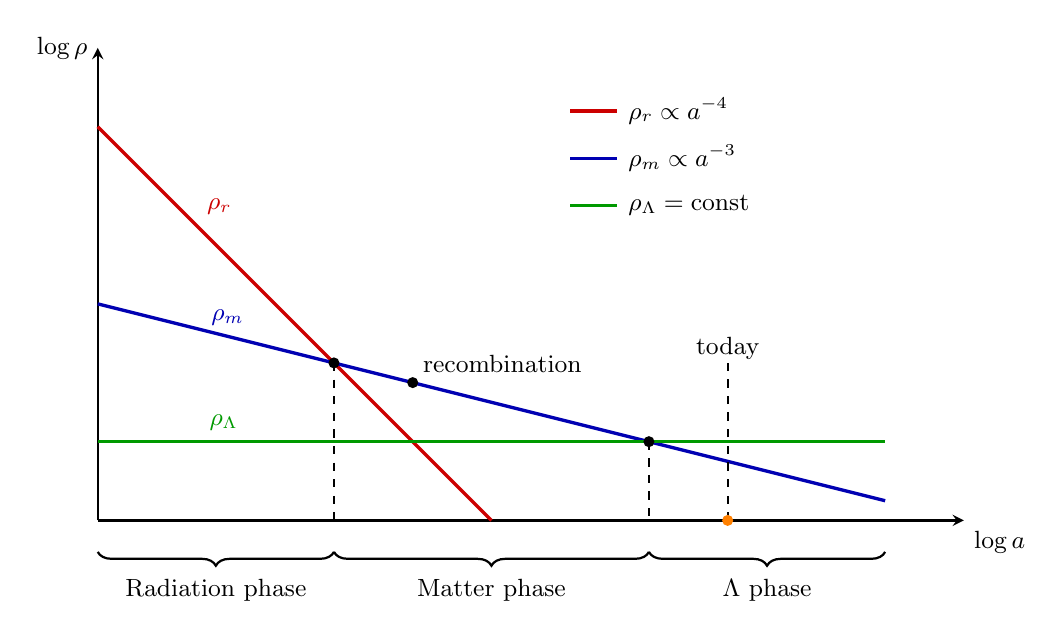
\begin{tikzpicture}[
    >=stealth,
    thick,
    font=\small,
    every node/.style={font=\small}
]

  % --- axes ------------------------------------
  \draw[->] (0,0) -- (11,0) node[below right] {$\log{a}$};
  \draw[->] (0,0) -- (0,6)  node[left] {$\log{\rho}$};

  % --- equality & recombination coordinates --------------------
  \coordinate (aeq)  at (3,2);   % matter–rad equality
  \coordinate (alam) at (7,1);   % matter–Λ equality
  \coordinate (rec) at (4,1.75);   % recombination

  % --- density curves --------------------------
  % radiation  ρ_r  (passes through (0,5) and (3,2))
  \draw[red!80!black, very thick] (0,5) -- (5,0)
      node[pos=.25,above right] {$\rho_r$};

  % matter      ρ_m  (line through (0,2.75) –> (7,1))
  \draw[blue!70!black,very thick] (0,2.75) -- (10,0.25)
  node[pos=.165,above] {$\rho_m$};

  % cosmological constant ρ_Λ
  \draw[green!60!black, very thick] (0,1) -- (10,1)
        node[pos=0.16,above] {$\rho_\Lambda$};

  % --- equality points & guides ----------------
  \fill (aeq)  circle (2pt);
  \fill (alam) circle (2pt);
  \fill (rec) circle (2pt);

  \draw[dashed] (aeq)  -- ++(0,-2);
  \draw[dashed] (alam) -- ++(0,-1);

  \draw (rec) node[above right] {recombination};

  % --- “today” marker --------------------------
  \draw[dashed] (8,0)  -- (8,2) node[above=-2.4pt] {today};
  \fill[orange] (8,0)  circle (2pt);

  % --- phase braces ----------------------------
  \draw[decorate,decoration={brace,mirror,amplitude=5pt}]
        (0,-0.4) -- (3,-0.4) node[midway,below=6pt] {Radiation phase};

  \draw[decorate,decoration={brace,mirror,amplitude=5pt}]
        (3,-0.4) -- (7,-0.4) node[midway,below=6pt] {Matter phase};

  \draw[decorate,decoration={brace,mirror,amplitude=5pt}]
        (7,-0.4) -- (10,-0.4) node[midway,below=6pt] {$\Lambda$ phase};

        % --- legend in top‐right corner ------------
  \begin{scope}[shift={(6,5)}]  % adjust (6,5) to taste
    \draw[red!80!black, very thick]   (0,0.2)   -- (0.6,0.2)   node[right, black] {$\rho_r\propto a^{-4}$};
    \draw[blue!70!black, very thick]  (0,-0.4) -- (0.6,-0.4) node[right, black] {$\rho_m\propto a^{-3}$};
    \draw[green!60!black, very thick] (0,-1) -- (0.6,-1) node[right, black] {$\rho_\Lambda=\mathrm{const}$};
  \end{scope}

\end{tikzpicture}
\end{center}
\subsection{Fine Tuning Problems in HBB}
%Horizon Problem
\begin{mycolorbox}
\textbf{Horizion problem:}

Observations tell us that the Universe is highly homogeneous and isotropic.
\begin{eqopt}[blue]
    \frac{\delta T}{T_{now}} \sim 10^{-4} - 10^{-5} \qquad T_{now} \approx 2.73 K
\end{eqopt} 
\underline{Assume $k=0$} in the metric. Rewrite~\eqref{00}~\eqref{11}. Consider a radial photon. 
Assume an initial singularity: $t_i = 0$, $a(t_i)=0$. Find \textcolor{darkgreen}{\textit{comoving particle horizon}}
\begin{equation}
    \Delta r = \int_0^t \frac{t^\prime}{a(t^\prime)} = \tau(t)-\tau(0)
\end{equation}
Use~\eqref{00}~\eqref{continuity} to relate proportionally $a$ and $t$. See that for $\omega>-1/3$ (SEC) $\Delta r$ is finite
$\Rightarrow$ \emph{there were regions not in causal contact in the past!}
Then compute the angle corresponding to the comoving horizon at recombination\footnote{Because CMB is emitted at that time! That's when the universe became transparent and photons were able to travel freely.} 
$\theta=(\tau_{rec}-\tau_{i})/(\tau_{now}-\tau_{rec})$.
Rewrite a general $\tau$ difference integrating and change variables to make $H$ appear so you can substitute with~\eqref{00}. \textcolor{blue}{$\theta \approx 1.15^\circ$}.
\end{mycolorbox}    

%Flatness Problem
\begin{mycolorbox}[red]
    \textbf{Flatness problem:}

    From current observations \textcolor{blue}{$\Omega_k <0.02$} $\Rightarrow$ one expects $\sum_i\Omega_i -1 \equiv \Omega_{tot}-1 \lesssim 10^{-2}$
    
    Compare present day to Plank epoch: 
    \begin{equation}
        \frac{\Omega_{tot}(t_{now})-1}{\Omega_{tot}(t_{P})-1} = \frac{(aH)^2|_{t_P}}{(aH)^2|_{t_{now}}}
    \end{equation}
    employ
    \begin{eqopt}[blue]
        \textcolor{darkred}{a \propto T^{-1}\footnote{Holds for radiation dominated Universe only, where $a \propto \rho^{-1/4}$ and \textcolor{darkred}{$\rho \propto T^4$ for black body radiation} }}
        \qquad H(t_P) \sim M_P \qquad T_P \sim M_P  \qquad H_{now}\sim 10^{-60}M_P 
    \end{eqopt}
    \emph{This means $\Omega_{tot}(t_P)-1 \lesssim 10^{-60}$ which would be highly fine-tuned}.
\end{mycolorbox}

\subsection{The actual problem: \textit{aH(t)}}
It all comes down to $aH$ being a decreasing function of time. ($1/aH$ is the \textcolor{darkgreen}{\textit{Hubble radius}})

Use~\eqref{00}~\eqref{continuity} to relate proportionally $a$ and $t$. Then relate $aH$ and $t$, include multiplicative $omega$ factors!. Finally, relate  $aH$ and $a$. 
See that SEC ($\omega>-1/3$) must be violated to have $aH$ increasing. \textcolor{darkred}{$\tau \in \interval[open right]{0}{\infty}$} , violating SEC we can push the singularity to $\tau_i = -\infty$.

%Horizon Problem
\begin{mycolorbox}
    \textbf{Equivalent conditions to $\omega<-1/3$:}

    \begin{enumerate}
        \item Decreasing comoving horizon
        \item Accelerated expansion: $\ddot{a} >0$
        \item Slowly varying $H$ \hfill \textcolor{darkgreen}{$\epsilon_H \equiv -\frac{\dot{H}}{H^2}$}\textcolor{mypurple}{$=3/2 (1+\omega)$} $\quad\Rightarrow \quad\epsilon < 1$
        \item Negative pressure
    \end{enumerate}
\end{mycolorbox}    

\begin{center}
    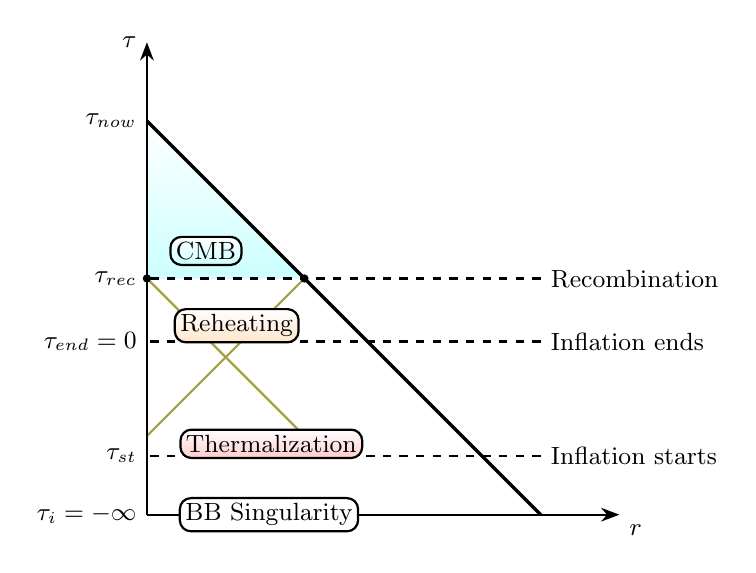
\begin{tikzpicture}[>=Stealth,thick,x=1cm,y=1cm,font=\small]

        %-------------------------------------------------
        % key coordinates
        %-------------------------------------------------
        \coordinate (tau0)   at (0,4);       % today
        \coordinate (tauEqL) at (0,2);       % τ_eq on axis
        \coordinate (tauEqR) at (2,2);       % τ_eq on light‑cone
        \coordinate (BB)     at (0,-1);      % Big‑Bang (origin of r axis)
        \coordinate (botR)   at (5,-1);      % bottom right on light‑cone
      
        %-------------------------------------------------
        % cyan path CMB
        %-------------------------------------------------
        \path[fill=cyan!20,shade, top color=white,bottom color=cyan!20,line width=1pt]
        (tau0) -- (tauEqR) -- (0,2) -- (tau0) -- cycle;
        \draw[yellow!60!black] (tauEqL) -- (2,0);
        \draw[yellow!60!black] (0,0)     -- (tauEqR); 
        
        %-------------------------------------------------
        % axes
        %-------------------------------------------------
        \draw[->] (0,-1) -- (6,-1) node[below right] {$r$};     % r‑axis
        \draw[->] (0,-1)  -- (0,5) node[left] {$\tau$};        % τ‑axis
      
        %-------------------------------------------------
        % past light‑cone boundary (grey)
        %-------------------------------------------------
        \draw[black,very thick] (tau0) -- (botR);
      
        % dashed horizontal guides
        \draw[dashed] (5,2) -- (0,2) node[left] {$\tau_{rec}$};; 
        \draw[dashed] (5,1.2) -- (0,1.2) node[left] {$\tau_{end}=0$};
        \draw[dashed] (5,-0.25) -- (0,-0.25) node[left] {$\tau_{st}$};
      
        %-------------------------------------------------
        % markers
        %-------------------------------------------------
        \fill (tauEqL) circle (1.5pt);
        \fill (tauEqR)     circle (1.5pt);

        \draw node[left] at (tau0) {$\tau_{now}$};
      
        \draw node[right] at (5,2) {Recombination};

        \draw node[right] at (5,1.2) {Inflation ends};

        \draw node[right] at (5,-0.25) {Inflation starts};
        
        %-------------------------------------------------
        % label boxes
        %-------------------------------------------------
        \node[draw,rounded corners,fill=white,inner sep=2pt]
              at ($(BB)+(1.55,0)$) {BB Singularity};

        \node[draw,rounded corners,fill=cyan!20,shade,
              top color=white,bottom color=cyan!20,inner sep=2pt]
              at ($(tauEqR)+(-1.25,0.35)$) {CMB};

        \node[draw,rounded corners,fill=red!20,shade,
              top color=white,bottom color=red!20,inner sep=2pt]
              at (1.58,-0.1) {Thermalization};   
        
        \node[draw,rounded corners,fill=orange!20,shade,
              top color=white,bottom color=orange!20,inner sep=2pt]
              at (1.14,1.4) {Reheating};       
      
        %-------------------------------------------------
        % τ_i  (inflation era)
        %-------------------------------------------------
        \node[left] at (0,-1) {$\tau_i = -\infty$};
      
      
      \end{tikzpicture}
\end{center}
How much do we need to push back in time $\tau_i$ so that the whole observable universe could have been in causal contact and thus thermalize?

At the onset of inflation assume an universe with far from flat initial conditions: $\Omega_k \sim 1 \Rightarrow \Omega_k(t_{st})/\Omega_k(t_{now})\gg 1$, rewrite and insert $aH(t_{end})/aH(t_{end})$. 
$H$ is nearly constant during inflation, \textcolor{darkgreen}{$N\equiv \log{a}$}. With $\frac{a_{end}}{a_{st}}= N_{tot}> 66+ \log{HT^{-1}(t_{end})}$ the flatness problem is solved. Usually, \textcolor{darkred}{\emph{one requires inflation to last 50-60 e-foldings}}.

% Clarifications
\begin{mycolorbox}[blue!30!black]
      \textbf{Subtle clarifications:}
  
\begin{enumerate}
      \item \textbf{What caused inflation?}
             Whatever it is that drives inflation it must have negative pressure. Thus it cannot be matter or radiation.
             Neither can be a cosmological constant because it would lead to perpetual rapid inflation (a cosmological constant does not diminish or evolve with time)~\cite{ModernCosm}.
  
             Simplest possibility is via the potential energy of a scalar field $\phi$ (there
             is no known scalar field that can drive inflation). It must have negative pressure and this requirement leads to potential energy dominating over kinetic energy.
      \item \textbf{Why is $H$ const during inflation?} The equation of state for the scalar field gives $\omega \sim -1$. This leads to $H$ being constant. When $\phi$ finishes its roll down the potential, $\omega$ becomes positive and $H$ starts to decrease. This is the end of inflation.
      \item \textbf{Is $a \propto T^{-1}$ valid in every epoch?} It always holds for $T$ being the temperature of radiation. Beware that $T$ is not the temperature of the Universe in every epoch.
  \end{enumerate}
\end{mycolorbox}
\begin{figure}[h]
      \centering
      \begin{tikzpicture}
        \node[anchor=south west,inner sep=0] (image) at (0,0) {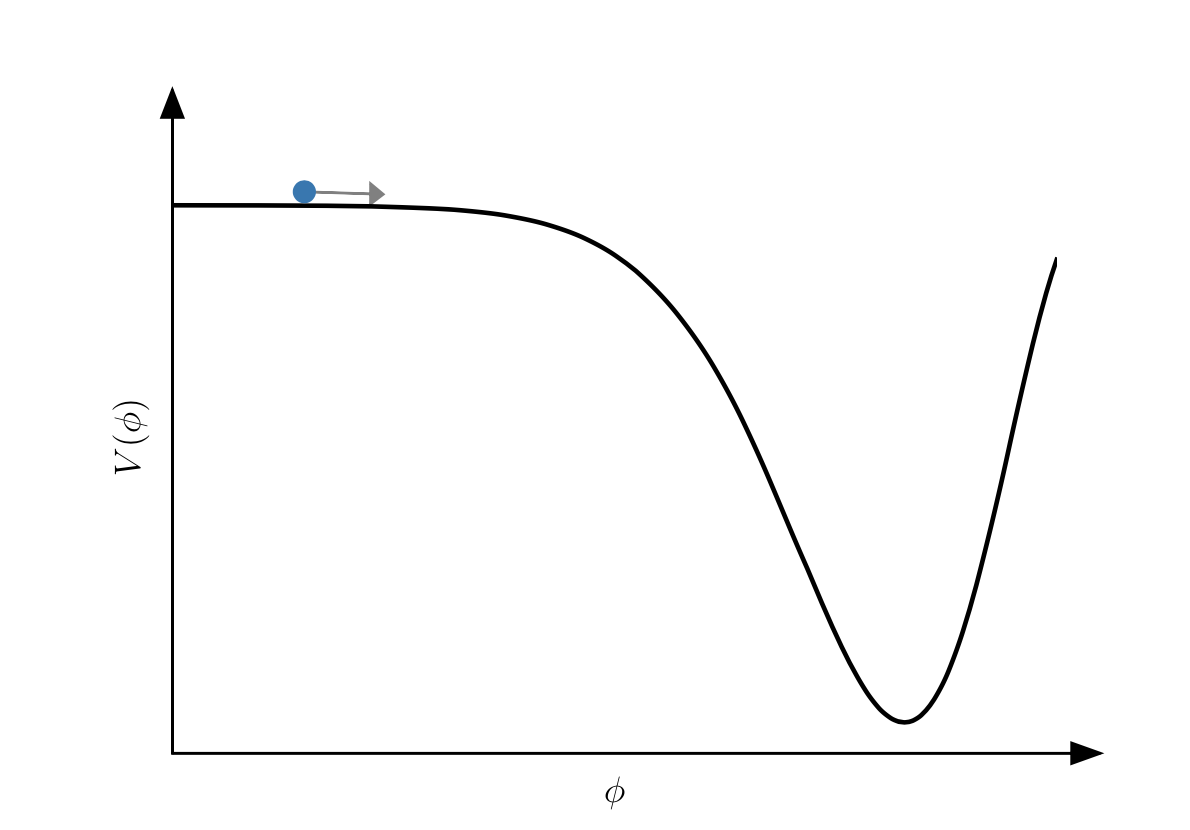
\includegraphics[width=0.8\textwidth]{Graphics/slow-roll.png}};
        \begin{scope}[x={(image.south east)},y={(image.north west)}]
          % Coordinates go from (0,0) bottom-left to (1,1) top-right
          % dashed horizontal guides
          \draw[dashed] (0.76,0.1) -- (0.76,0.8) node[above] {Inflation ends}; 
        \end{scope}
      \end{tikzpicture}
      \caption{A scalr field rolling down a potential~\cite{ModernCosm}.}
  \end{figure}

\newpage
\section{Theories of Inflation}\label{sec:section2}
\subsection{}
\subsection{$P(X,\phi)$ theories}\label{sec:Pxphi}
\textcolor{darkgreen}{$X \equiv 1/2(\partial_{\mu} \phi)^2 \qquad E \equiv 2XP_X -P$}. Action for $P(X,\phi)$ theories is 
\begin{eqopt}
    S = \int d^4x \sqrt{g}\left[\frac{M_P^2}{2} R + P (X,\phi)\right]
\end{eqopt}
Equations of motion for $g^{\mu\nu}$ and $\phi$ are
\begin{equation}
    H^2 = \frac{1}{3M_P^2}E \qquad \dot{E} = -3H\left(E+P\right)
\end{equation}
Find expression for $\epsilon$ and condition for $\epsilon \ll 1$.

In fluid mechanics the speed of sound is defined as a derivative of the pressure with
respect to the density at fixed entropy per particle:
\textcolor{darkgreen}{$c_s^2 = \frac{\partial P}{\partial \rho}\big|_{s/n}$} .
It is the velocity at which adiabatic compression and rarefaction waves propagate
in a medium~\cite{piattellaNoteThermodynamicsSpeed2014}.
\begin{equation}
    c_s^2 = \frac{P_X dX + P_\phi d\phi}{\rho_X dX + \rho_\phi d\phi}\Bigg|_{s/n} = \frac{P_X}{\rho_X} = \frac{P_{X}}{P_X + 2XP_{XX}}
\end{equation}
As one can prove that $d(s/n)=0$ is equivalent to $d\phi = 0$. In our context, $c_s$ is the speed of scalar perturbations.

%K-Inflation models
\begin{mycolorbox}[orange!50!black]
    \textbf{K-Inflation models:}

    Effective kinetic Lagrangian can be written as
    \begin{eqopt}
        \mathcal{L} \supset  \sum_{n\geq1}  f(\phi)\frac{X^n}{\Lambda^{4n-4}} 
    \end{eqopt}
$\Lambda$ is the cut-off scale of the effective field theory because $\Lambda^4 \gg X$ kills everything execpt the first term, which is the one of slow roll inflation.
But there are potential problems with ghosts and radiative stability.
\end{mycolorbox}    
%DBI Inflation
\begin{mycolorbox}[orange!50!black]
    \textbf{Dirac-Born-Infeld Inflation:}

    It is a model of inflation based on the Dirac-Born-Infeld (DBI) action, which describes the dynamics of a D-brane in string theory. 
    \begin{eqopt}
        S = -\int d^4x \sqrt{g} \left[ \frac{1}{f(\phi)} \sqrt{1 + f(\phi) \partial_\mu\phi\partial^\mu\phi} - \frac{1}{f(\phi)} + V(\phi) \right]
    \end{eqopt}
    The DBI action includes a kinetic term that is non-linear in the field velocity, leading to a speed limit on the field's motion (due to $\sqrt{\dots}$). This non-linear kinetic term can give rise to an effective sound speed that is less than one (which is constrained by observations!), allowing for a more gradual roll of the inflaton field and potentially addressing issues related to the generation of primordial perturbations.
\end{mycolorbox}    
\newpage

\section{Quantum Inflation}\label{sec:section3}
\emph{When inflation ends the inflaton dumps its energy into standard model particles:} this is the process called \textit{reheating}. 
After reheating the Universe is still radiation dominated until recombination at $t_{eq}$. The latter time can be estimated, in terms of redshift $z_{eq}$, by $\rho_m^{eq} = \rho_\gamma^{eq}$ and then employing $\Omega_{\rho_i}^{\text{now}}$.

After radiation-matter equivalence the Universe remains a coupled baryon-photon plasma until recombination, when the already existing free photons can propagate freely; resulting in Plankian spectrum we observe: the CMB.

To estimate $z_{rec}$ start from the number density of a certain species
\begin{eqopt}[darkred] \label{eq:NumberDensityExact}
    n=\frac{g}{(2\pi)^3}\int f(\mathbf{p}) d^3p \; \textcolor{black}{=\, \frac{g}{2\pi^2}\int_m^\infty f(\mathbf{E}) E \sqrt{E^2-m^2} dE} \qquad f(\mathbf{p})= \frac{1}{e^{\frac{E-\mu}{T}}\pm 1}
\end{eqopt}
Approx $e^{\frac{E-\mu}{T}}\pm 1 \approx e^{\frac{E-\mu}{T}}$ and consider non-relativistic particles, for which $T\ll m$:
\begin{eqopt}[darkred]\label{eq:NumberDensityApprox}
    n=g\left(\frac{mT}{2\pi}\right)^{3/2}\,e^{\frac{\mu - m}{T}}
\end{eqopt}
$g = 2 S +1$-factors are the usual internal degeneracy (spin, etc.) of each species.
The \textit{proton-electron capture} to form neutral hydrogen is the process happening at recombination. In the early Universe before recombination we have equilibrium: $p + e \leftrightarrow  H + \gamma$.
\underline{Assume $n_B = n_p + n_H$}, i.e.\ all baryons are in the form of protons and hydrogen atoms. \underline{Assume thermal and chemical ($\mu_H = \mu_p + \mu_e$) equilibrium}. Furthermore, $n_p = n_e$ due to charge neutrality.
We are interested in the ratio $n_H / (n_p n_e) $ as it tells us how neutral (and thus transparent for photons) is the Universe at temperature $T$. Define \textit{hydrogen biding energy} \textcolor{darkgreen}{$B\equiv m_p+m_e -m_H$}. Employing~\eqref{eq:NumberDensityApprox}
\begin{equation}\label{eq:SahaInitial}
    \frac{n_H}{n_pn_e}\, \overset{m_H \simeq m_p}{\approx}\, \underbrace{\frac{g_H}{g_p g_e}}_{=1} \left(\frac{2\pi}{m_e T}\right)^{3/2} e^{B/T} \overset{!}{=} \frac{n_p /n_B^2}{n_e^2/n_B^2} = \frac{1}{n_B} \frac{1-n_e/n_B}{n_e^2/n_B^2}
\end{equation}
Define the \textit{fractional ionization} \textcolor{darkgreen}{$ \chi_e \equiv n_e / n_B$} and the \textit{baryon to photon ratio} \textcolor{darkgreen}{$ \eta \equiv n_B / n_\gamma$}\textcolor{blue}{$\,\simeq 6\cdot 10^{-10}$}. Where \textcolor{darkred}{$n_\gamma = \frac{2}{\pi^2} \zeta(3)T^3$} comes from direct integration of~\eqref{eq:NumberDensityExact}.
We can now rewrite~\eqref{eq:SahaInitial} in the form called \textit{Saha equation}
\begin{eqopt}\label{eq:Saha}
    \frac{1-\chi_e}{\chi_e^2}\Bigg|_{eq} = \frac{4\sqrt{2}}{\sqrt{\pi}}\zeta(3) \eta \left(\frac{T}{m_e}\right)^{3/2} e^{B/T}
\end{eqopt}
Universe becomes transparent for $\chi_e \rightarrow 0$, as free protons and electrons diminish and the former start having a  high mean free path.
\textcolor{darkred}{For $\chi_e = 0.01$ we have from~\eqref{eq:Saha} $T \approx 3500K$} $\; \Rightarrow z_{rec}=\frac{T_{rec}}{T_{now}}-1 \simeq 1200$.

Thermal equilibrium is no longer a good approximation during inflation, indeed a more accurate result can be found using kinetic theory: \textcolor{darkred}{$z_{rec}\simeq1100$}.

\subsection{Scalar field in dS space-time}\label{sec:dS}
Use conformal time in the metric. Cosnider a real, minimally coupled scalar field $\phi(x^\mu)$:
\begin{eqopt}
    S=\frac{1}{2}\int d^4x \sqrt{-g} \left( \partial_\mu \phi \partial^\mu \phi -  m^2 \phi^2 \right)
\end{eqopt}
Rescale with \textcolor{darkgreen}{$\chi \equiv a \phi$} and eventually define \textcolor{darkgreen}{$m_{\text{eff}}^2 \equiv m^2a^2-\frac{a^{\prime\prime}}{a}$}
Action is explicitly time dependent $\Rightarrow$ energy not conserved $\Rightarrow$  particle creation (with energy supplied by the classical gravitational field).
Get EOM for $\chi$, then expand in Fourier modes:
\begin{eqopt}
    \chi(\mathbf{x},\tau) = \int \frac{d^3k}{(2\pi)^{3/2}} \chi_{\mathbf{k}}(\tau) e^{i\mathbf{k}\cdot\mathbf{x}} \label{Fourier}
\end{eqopt}
Rewrite EOM in terms of $\chi_{\mathbf{k}}$. Note that $\chi$ is a real number $\Rightarrow \chi_{\mathbf{k}}^* = \chi_{-\mathbf{k}}$. EOM just depends on $\abs{\mathbf{k}}$, general solution is
\begin{eqopt}[darkred]\label{Mode_exp}
    \chi_{\mathbf{k}}(\tau) = \frac{1}{\sqrt{2}} \left( a^-_{\mathbf{k}} \, v^*_k(\tau) + a^+_{-\mathbf{k}}\, v_k(\tau)  \right) 
\end{eqopt}
\emph{$a_{\mathbf{k}}$ coefficients are not yet identified as annihilation/creation operators, $v_k$ are called mode functions.} Normalization is \textcolor{darkred}{$\Im(v^{\prime}v^*)=1/2$}. 
Put back in~\eqref{Fourier}
\begin{equation}\label{Fourier_v}
\chi(\mathbf{x}, \tau) = \frac{1}{\sqrt{2}} \int \frac{d^3 k}{(2\pi)^{3/2}} \left[ a^-_{\mathbf{k}} v_k^*(\tau) e^{i \mathbf{k} \cdot \mathbf{x}} + a_{-\mathbf{k}}^+ v_k(\tau) e^{-i \mathbf{k} \cdot \mathbf{x}} \right]
\end{equation}
EOM for $v_k$ is
\begin{equation}
    v_k^{\prime\prime} + \overbrace{\left( k^2 + m_{\text{eff}^2} \right)}^{\omega_k^2} v_k = 0
\end{equation}

Define canonical momentum and Hamiltonian:
\begin{eqopt}[darkgreen]
\Pi = \frac{\partial \mathcal{L}}{\partial \chi'} \qquad \hat{\mathcal{H}} = -\mathcal{L} + \hat{\Pi} \chi'
\end{eqopt}
Impose equal time commutation relations: $[\hat{\chi}(x, \tau), \hat{\Pi}(y, \tau)] = i \delta^3(x - y)$

Here one may show that, promoting the coefficients $a_{\mathbf{k}}$ to operators, they obey commutation relations of annihilation/creation operators; with which one can construct quantum states of the theory.
\begin{equation}
    \ket{m_{\mathbf{k_1}}, n_{\mathbf{k_2}}, \ldots} = \frac{1}{\sqrt{m!n!\ldots}}(\hat{a}_{\mathbf{k}_1}^\dagger)^m(\hat{a}_{\mathbf{k}_2}^\dagger)^n\ldots \ket{0}
\end{equation}

%Bogoliubov transformation
\begin{mycolorbox}[red!50!orange]
    \textbf{Bogoliubov transformation:}

\begin{eqopt}
    u_k(\tau) = \alpha_k v_k(\tau) + \beta_k v^*_k(\tau)
\end{eqopt}
Impose normalization condition on $u_k$: $u_k^{\prime}u_k^* - u_k^{\prime *}u_k=i$ to get \textcolor{darkred}{$\abs{\alpha_k}^2 - \abs{\beta_k}^2 = 1$}.
\begin{equation}\label{Fourier_u}
    \chi(\mathbf{x}, \tau) = \frac{1}{\sqrt{2}} \int \frac{d^3 k}{(2\pi)^{3/2}} \left[ b^-_{\mathbf{k}} u_k^*(\tau) e^{i \mathbf{k} \cdot \mathbf{x}} + b_{-\mathbf{k}}^+ u_k(\tau) e^{-i \mathbf{k} \cdot \mathbf{x}} \right]
    \end{equation}
To find relation between $b_{\mathbf{k}}$ and $a_{\mathbf{k}}$, equate~\eqref{Fourier_v} and~\eqref{Fourier_u}
A generic state is 
\begin{equation}
    \ket{\psi} = \sum_{m,n,\ldots} C_{mn}^A \ket{m_{\mathbf{k_1}}, n_{\mathbf{k_2}}, \ldots}_A = \sum_{m,n,\ldots} C_{mn}^B \ket{m_{\mathbf{k_1}}, n_{\mathbf{k_2}}, \ldots}_B
\end{equation}
Show that \textcolor{red}{$\tensor[_B]{\langle0|}{}\,\hat N^A_{\mathbf k}\,\ket{0}_{B} = \abs{\beta_{\mathbf{k}}}^2 \delta^{(3)}(0)$}, divergence is due to infinite spatial volume.
\end{mycolorbox}

%Flat quantization
\begin{mycolorbox}[green!50!black]
    \textbf{Flat background:}
    
\emph{Hamiltonian is time independent. The vacuum is the eigenstate of the $\hat{H}$ with lowest energy.}
Substitute~\eqref{Mode_exp} in $\hat{H}$ (here $a=0 \Rightarrow m_{\text{eff}}=0$) and define 
\begin{eqopt}[darkgreen]
    F_k \equiv v_k^{\prime 2} +k^2 v_k^2 \qquad E_k \equiv  \abs{v_k^{\prime}}^2 +k^2 \abs{v_k}^2
\end{eqopt}
Write the mode functions as $v_k = r_k(\tau) e^{i\alpha_k(\tau)}$. Impose normalization condition on $v_k$ to rewrite $E_k$ and then minimize it: $dE_K/dr^\prime = 0 , dE_K/dr = 0 $. Find 
\begin{equation}\label{eq:flat_vk}
    v_k = \frac{1}{\sqrt{2k}} e^{ik\tau}
\end{equation}
Use it to simplify the Hamiltonian as $E_k,F_k$ take much simpler forms.
\end{mycolorbox} 

%dS quantization
\begin{mycolorbox}[green!50!orange]
\textbf{dS background:} \hfill $\rho=T^{00}=\Lambda/8\pi G=-T^{ii}=-P \Rightarrow H^2 = \text{const}$

\vspace{1mm}
Let \textcolor{mypurple}{$k^2\rightarrow \omega^2_k=k^2+m_{\text{eff}}^2$} 
\begin{equation}
    v_k(\tau_0) = \frac{1}{\sqrt{2\omega_k(\tau_0)}} e^{i\omega_k(\tau_0)\tau_0} 
\end{equation}
\emph{To these one can associate a vacuum state $\ket{0}_{\tau_0}$, which is the eigenstate of the annihilation operator $\hat{a}_{\mathbf{k}}$ at time $\tau_0$. It will not be the 
lowest energy state at later times $\rightarrow$ time dependence of the effective mass gives rise to particle creation.}

In $dS$ spacetime $a\propto e^{Ht} \; \Rightarrow\; \tau = \int_{-\infty}^t dt e^{-Ht}\; \Rightarrow\;  \tau  = -1/aH \; \Rightarrow\;  \tau \in \ointerval[scaled]{-\infty}{0} \; \Rightarrow \; m_{\text{eff}}=(aH)^2\left[(m/H)^2-2\right]$
EOM for $v_k$ becomes 
\begin{equation}\label{eq:EOMvk}
    v_k^{\prime\prime} + \Biggl[ k^2 - \frac{1}{\tau^2}\overbrace{\left(2-\frac{m^2}{H^2}\right)}^{\nu^2-1/4} \;\Biggr] v_k = 0
\end{equation}
Solution is in terms of Hankel functions:
\begin{eqopt}[darkred]
    v_k(\tau) = \sqrt{-\tau}\left[ C_1 H_\nu^{(1)}(-k\tau)+ C_2 H_\nu^{(2)}(-k\tau) \right]
\end{eqopt}
with \textcolor{darkgreen}{$\nu \equiv \sqrt{\frac{9}{4}-\frac{m^2}{H^2}}$}. \underline{Consider massless scalar field} $\Rightarrow \nu = 3/2$. This leads to
\begin{eqopt}[darkred]\label{mode_dS}
    v_k(\tau) = \left[ C_1\left(1-\frac{i}{k\tau}\right)+ C_2 \left(1+\frac{i}{k\tau}\right) \right]
\end{eqopt}
Now impose initial conditions at $\tau\ll 1$ to determine $C_1$ and $C_2$: \emph{ask the scalar to be in the instantaneous vacuum state at early times} $\Rightarrow$ $C_1=0$ and $C_2=1$ (due to limit forms of $H_\nu^{(1,2)}$) to recover the flat space limit~\eqref{eq:flat_vk}.
Note that, at early times, $k \gg 1/\tau$ as $k$ is a fixed mode\footnote{A mode $k$ is associated with a wavelength \textcolor{darkred}{$\lambda = 2\pi/k$}, so when a mode $k</>aH$, it is said to be super/sub-horizon meaning that the wavelength is larger/smaller than the Hubble radius}.

The mode functions in~\eqref{mode_dS} define the \textit{\textcolor{darkgreen}{Bunch-Davies vacuum}} $\ket{0}_{BD}$, i.e. the vacuum state at $\tau_0$.
\begin{center}
    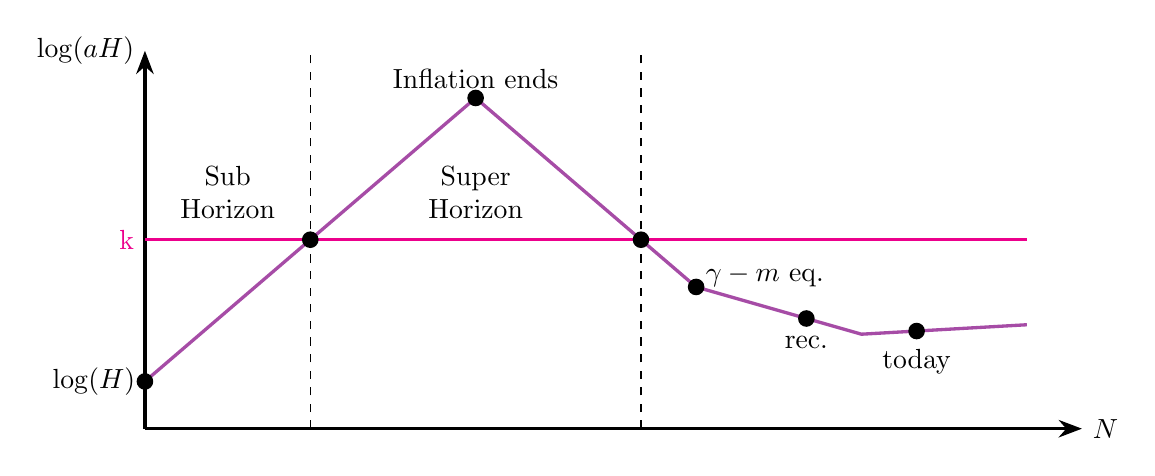
\begin{tikzpicture}[x=1.4cm,y=1.2cm]

        % --- axes -----------------------------------------------------
        \draw[very thick,->] (0,0) -- (0,4) node[below,left] {$\log(aH)$};
        \draw[very thick,->] (0,0) -- (8.5,0) node[right] {$N$};
      
        % --- horizon‐crossing “grid” (magenta) ------------------------
        \coordinate (khoriz) at (1.5,0);
        \coordinate (lhoriz) at (0,2);
      
        \draw[dashed] (khoriz) ++(0,0) -- ++(0,4);   % vertical
        \draw[dashed] (khoriz) ++(3,0) -- ++(0,4);   % vertical
        \draw[magenta,very thick]  (8,2) -- (lhoriz) node[left] {k};  % horizontal

         % --- illustrative k-mode trajectory (lavender) ----------------
         \draw[very thick,violet!70!white] 
         plot coordinates{(0,0.5) (3,3.5) (5,1.5) (6.5,1) (8,1.1)};
      
        % intersection dots 
        \fill (1.5,2) circle (3pt);
        \fill (4.5,2) circle (3pt);
        \fill (0,0.5) circle (3pt);
        \fill (3,3.5) circle (3pt) node[above] {Inflation ends};
        \fill (5,1.5) circle (3pt) node[above=4pt,right] {$\gamma-m$ eq.};
        \fill (6,1.166) circle (3pt) node[below=3pt] {rec.};
        \fill (7,1.03333) circle (3pt) node[below=3pt] {today};
      
        % --- sub-/super-horizon labels --------------------------------
        \node[align=center] at (0.75,2.5) {Sub\\Horizon};
        \node[align=center] at (3,2.5) {Super\\Horizon};

        % log(H) marker
        \draw node[left] at (0,0.5) {$\log(H)$};
      
      \end{tikzpicture}
\end{center}

The physical wavelength is defined as \textcolor{darkgreen}{$\lambda_{\text{phys}} = a \lambda$}. 
For de Sitter space, $\textcolor{darkred}{R_{dS}= 12H^2} \; \Rightarrow \; \abs{k\tau} \propto R_{dS}/\lambda_{\text{phys}}$, 
imposing $\ll 1$ we find that \emph{background curvature is much grater than the physical wavelength of the mode $\Rightarrow$ at early times modes behave as they were in Minkowski spacetime}.

One can then calculate observables like the \textit{power spectrum} $\tensor*[_{BD}]{\expval{0|\hat \chi_{\mathbf{k}}\,\hat \chi_{\mathbf{k}'}|0}}{_{BD}} = \textcolor{darkgreen}{P_{v_k}}\delta(\mathbf{k}+\mathbf{k}')$, which is $\approx (aH)^2/(2k^3)$ for $\abs{k\tau} \ll 1$ (measuring $P_{v_k}$ one can get $aH$!)
\end{mycolorbox} 


\subsection{Cosmological Perturbation Theory}
\label{sec:cosmological_perturbation_theory}
The zeroth-order scheme outlined
in Section~\ref{sec:slowRollInfl} ensures that the universe will be close to uniform on all scales of
interest today. There are perturbations about this zeroth-order scheme, though, and these
perturbations—produced early on when the scales are causally connected—persist long
after inflation has terminated.

In cosmology, we always work in terms of statistics, such as the correlation function
and power spectrum, because no known theory predicts the overdensity in a given spot
on the sky. In the inflationary scenario, this uncertainty is fundamental: inflation erases all
traces of what came before it, and replaces those with quantum-mechanical vacuum fluctuations, 
which cannot be predicted in principle. What inflation predicts then is precisely
the statistical distributions from which the perturbations are drawn.

We are most interested in scalar perturbations to the metric since these couple to the
density of matter and radiation and ultimately are responsible for the structure we observe
in the universe. Inflation also generates tensor fluctuations in the metric, that is, gravitational
waves. These are not coupled to the density and so are not responsible for the large-scale structure 
of the universe, but they do induce anisotropies in the
CMB~\cite{ModernCosm}.

\begin{eqopt}\label{perturbation}
    g_{\mu\nu} = \bar{g}_{\mu\nu} + \delta g_{\mu\nu} \qquad T_{\mu\nu} = \bar{T}_{\mu\nu} + \delta T_{\mu\nu}
\end{eqopt}
Expanding the Einstein equations to first order in perturbations, we have:
\begin{equation}
    \delta G_{\mu\nu} = 8\pi G \, \delta T_{\mu\nu},
\end{equation}
\emph{Write down the most general linear perturbation that is compatible with the spatial symmetries of an FRW background, 
and then decompose every spatial object into irreducible pieces.} Background is homogeneous and isotropic $\rightarrow$ spatial rotations 
(plus translations) act as a symmetry group. Irreducible representations of $SO(3)$ are labelled by spin: 0 scalars, 1 vectors and 2 tensors. Use conformal time in the metric.
\begin{eqopt}\label{eq:fullMetric}
    \frac{ds^2}{a^2} = \left(1 + 2\Phi\right) d\tau^2 +2\left(B_{,i} + S_{i}\right)  d\tau dx^i - \left[(1 - 2\Psi)\delta_{ij} -2 E_{,ij} -F_{i,j}-F_{j,i}- h_{ij}\right ]  dx^i dx^j 
\end{eqopt} \vspace{-5mm}
\begin{eqopt}\label{eq:metricPT}
\delta g_{00} = 2a^2 \Phi \qquad \delta g_{0i} = a^2 \left(B_{,i} + S_i\right)\qquad \delta g_{ij} = a^2 \left(2\Psi \delta_{ij}+2E_{,ij}+F_{i,j}+F_{j,i}+ h_{ij}\right) 
\end{eqopt}
$S_i$, $F_i$ and $h_{ij}$ are transverse because they come from the decomposition of $V_i= \partial_i V + V^{\perp}_i$ and $W_{ij}=W\delta_{ij}+\partial_i\partial_j W+ \partial_i W_j + \partial_j W_i + W^{\perp}_{ij} = 0$ (Helmholtz theorem):
\begin{eqopt}[darkred]
    S^i_{,i} = 0 \qquad F^i_{,i} = 0 \qquad h^i_{j,i} =0 = h^i_i
\end{eqopt}
$\delta g_{\mu\nu}$ is symmetric thus has 10 d.o.f., indeed we have 4 scalar, 2 vector (with 2 d.o.f. each) and 1 tensor (with $3(3+1)/2 - 1 -3 = 2$ d.o.f.) perturbations: 10 functions specifying the perturbation. Not all are independent, though. 
The gauge freedom of the metric allows us to set some of them to zero\footnote{The gauge freedom of the metric is a consequence of the diffeomorphism invariance of GR. We can always choose a coordinate system in which the metric takes a certain form. This is called a gauge choice.}.

\begin{equation}
    x^\mu \rightarrow \tilde{x}^{\mu} = x^{\mu} + \xi^{\mu}(x) \qquad \text{gives} \qquad \tilde{g}_{\mu\nu}(\tilde{x}) = \frac{\partial x^\rho}{\partial\tilde{x}^\mu}\frac{\partial x^\sigma}{\partial\tilde{x}^\nu}g_{\rho\sigma}(x)
\end{equation}
From this and equation~\eqref{perturbation} you can see that the perturbation transforms as
\begin{equation}
    \delta \tilde{g}_{\mu\nu} = \delta g_{\mu\nu} - \tilde{g}_{\mu\nu,\sigma} \xi^\sigma - \tilde{g}_{\mu\sigma} \xi^\sigma_{,\nu} - \tilde{g}_{\nu\rho} \xi^\rho_{,\mu} 
\end{equation}
Expand $\xi^\mu = \left(\xi^0,\xi^i_\perp+\xi^{,i}\right)$ using Helmholtz decomposition. Find $\delta \tilde{g}_{00}, \delta \tilde{g}_{0i}, \delta \tilde{g}_{ii} $.   


%%Tensor Perturbations
%\begin{mycolorbox}[purple!30!red]
%    \textbf{Tensor perturbations:}  
%
%    \begin{equation*}
%        ds^2=a^2\left\{d\tau^2 - \left[\delta_{ij}+h_{ij}\right]dx^i dx^j\right\}
%        \end{equation*}
%    
%    $\tilde{h}_{ij} = h_{ij} \; \rightarrow \;$ gauge invariance.  
%\end{mycolorbox} 
\subsection{Hydrodynamical Perturbations}
\label{sec:hydrodynamical_perturbations}

Hydrodynamical perturbations are not gauge invariant, they are scalar perturbations:
\begin{equation*}
    ds^2=a^2\left\{\left(1+2\Phi\right)d\tau^2 +2B_{,i}dx^i d\tau - \left[\left(1-2\Psi\right)\delta_{ij}-2E_{,ij}\right]dx^i dx^j\right\}
\end{equation*}

Use $\delta \tilde{g}_{00}, \delta \tilde{g}_{0i}, \delta \tilde{g}_{ii} $ to find $\tilde{\Phi},\tilde{B},\tilde{\Psi},\tilde{E}$.
Then choose $\xi,\xi^0$ so that only two perturbations remain. \textit{Conformal Newtonian gauge} is \textcolor{blue}{E=B=0}.

%EMT Perfect Fluid
\begin{mycolorbox}[pink!70!red]
    \textbf{EMT of a perfect fluid:}

    Expand $\rho, P, u^{\mu}$ in terms of the background and perturbations. 
    
    $u^0 = \bar{u}^0+\delta u^0, \quad u^i= \frac{dx^i}{ds}= a^{-1}\delta v^i$, as (\textcolor{darkgreen}{$\delta v^i = \frac{dx^i}{d \tau}$}). Impose $\bar{u}^{\mu}\bar{u}_{\mu}=1$, and $u^{\mu}u_{\mu}=1$
    to get $u_0$ and $u^0$. At first order in perturbations obtain 
    \begin{eqopt}[darkred]\label{eq:variationsTPF}
        \delta T^0_0= \delta \rho \qquad \delta T^0_i=-\delta v_i \left(\bar{\rho}+\bar{P}\right) \qquad \delta T^i_j=-\delta^i_j \delta P
    \end{eqopt}
    Solve conservation equation $\nabla^\mu T_{\mu\nu}=0$ (employ zeroth order $\bar{\nabla}^\mu \bar{T}_{\mu\nu}=0$) in \textcolor{blue}{$\delta g_{0i}=0$} gauge 
    (because $B=0$ and I ignore $S_i$ as I am considering scalar perturbations!); to do so expand $\Gamma^{\rho}_{\mu\nu} = \bar{\Gamma}^{\rho}_{\mu\nu} + \delta \Gamma^{\rho}_{\mu\nu}$\footnote{$\delta \Gamma^\rho_{\mu\nu}= \frac{1}{2} g^{\rho \alpha}\left(\nabla_\mu \delta g_{\alpha \nu}+\nabla_\nu \delta g_{\alpha \mu}-\nabla_\alpha \delta g_{\mu \nu}\right)$}
    and define \textcolor{darkgreen}{$h_{\mu\nu}\equiv a^{-2}g_{\mu\nu}$} $\,\Rightarrow \, g_{\mu \nu} = \bar{g}_{\mu \nu} + a^2 h_{\mu\nu}$
    
    E.g. $\delta \Gamma^0_{00} \simeq \frac{1}{2}\bar{g}^{00}\left(\bar{\nabla}_0\delta g_{00}\right)= \frac{1}{2}\delta g^\prime_{00}\frac{1}{a^2}-\delta g_{00}\frac{a^\prime}{a^3}= \frac{1}{2}h_{00}^\prime$
    \begin{align}
        &\delta \rho' + 3 \frac{a'}{a} (\delta P + \delta \rho) + (\bar{P} + \bar{\rho}) (\partial_i \delta v^i - \frac{1}{2} h_i^{i\,\prime}) = 0 \label{eq:conservation1}\\
        &\partial_i \delta P + (\bar{P} + \bar{\rho}) \left( 4 \frac{a'}{a} \delta v_i + \frac{1}{2} \partial_i h_{00} \right) + \left[ \delta v_i (\bar{P} + \bar{\rho}) \right]' = 0
    \end{align}  

    If the Universe contains multiple non-interacting fluids, each one is conserved separately and these equations hold for each fluid component.
\end{mycolorbox}    

At first order the Einstein equations are
\begin{align}
    \delta G^0_0 &= \frac{2}{a^2} \left( -\Delta \Psi + 3 \frac{a'}{a} \Psi' - 3 \left( \frac{a'}{a} \right)^2 \Phi \right)  \overset{!}{=} 8 \pi G \delta T^0_0 = 8 \pi G \, \delta \rho_{\text{tot}} \\
    \delta G^0_i &= \frac{2}{a^2}  \left( -\partial_i \Psi' + \frac{a'}{a} \partial_i \Phi \right) \overset{!}{=} 8 \pi G \delta T^0_i = -8 \pi G \,  \delta v_i^{\text{tot}} (\bar{\rho}_{\text{tot}} + \bar{P}_{\text{tot}})\\ 
    \delta G^i_j &= \frac{1}{a^2} \partial^i\partial_j (\Phi + \Psi) - \frac{2}{a^2} \delta^i_j \Bigg[ -\Psi'' + \frac{1}{2} \Delta (\Phi + \Psi) + \frac{a'}{a} (\Phi' - 2 \Psi') + \frac{2 a''}{a} \Phi \nonumber \\
    &- \left( \frac{a'}{a} \right)^2 \Phi \Bigg] \overset{!}{=} 8 \pi G \delta T^i_j = -8 \pi G \, \delta^i_j \, \delta P_{\text{tot}} \label{eq:ij}
\end{align}
From~\eqref{eq:ij} taking a component with $i\neq j$ we find $\Phi = -\Psi$. Use this and \textcolor{darkred}{$\delta v_i = \partial_i \delta v$}\footnote{You still have residual gauge freedom on $\xi_i^\perp$ to set $\delta v^\perp_i=0$} to simplify the equations.
Recalling $h_{\mu\nu}$ is related to $\Phi$ by~\eqref{eq:metricPT}, \emph{you have 5 single fluid component ($\lambda$) equations~\eqref{eq:conservation1} -~\eqref{eq:ij} and 4 variables: $\delta \rho_\lambda, \delta P_\lambda, \delta v_\lambda, \Phi$; not all are independent.}
Below they are rewritten (sometimes use the trick $\partial_i A=\partial_i B \,\Rightarrow \, A=B$)
\begin{align}
    &{\color{mypurple}\Delta \Phi - 3 \frac{a'}{a} \Phi' - 3 \left( \frac{a'}{a} \right)^2 \Phi = 4 \pi G \, a^2 \, \delta \rho_{\text{tot}}} \label{eq:hydro1} \\[1ex] 
    &\Phi' + \frac{a'}{a} \Phi = -4 \pi G \, a^2 \left[ (\bar{\rho} + \bar{P}) \delta v \right]_{\text{tot}} \\[1ex]
    &{\color{mypurple}\Phi'' + 3 \frac{a'}{a} \Phi' + 2 \frac{a''}{a} \Phi - \left( \frac{a'}{a} \right)^2 \Phi = 4 \pi G \, a^2 \, \delta P_{\text{tot}}} \label{eq:hydro3}\\[1ex]
    &\delta \bar{\rho}_\lambda^{\text{ }\prime} + 3 \frac{a'}{a} (\delta \rho_\lambda + \delta P_\lambda) + (\bar{\rho}_\lambda + \bar{P}_\lambda) \left( \Delta \delta v_\lambda - 3 \Phi' \right) = 0 \\[1ex]
    &\delta P_\lambda +\left[ (\bar{\rho}_\lambda + \bar{P}_\lambda) \delta v_\lambda \right]' + 4 \frac{a'}{a} (\bar{\rho}_\lambda + \bar{P}_\lambda) \delta v_\lambda + (\bar{\rho}_\lambda + \bar{P}_\lambda) \Phi = 0
\end{align}
Notice that $\Delta \equiv \nabla_i \nabla^i$ is the Laplacian operator in 3D space. For flat FRW spacetime $\Delta = \partial_i \partial^i$ because the connection is trivial as no metric terms depend on $x^i$.
\subsection{Single Component Fluid}\label{sec:SingCompFluid}

Take~\eqref{eq:hydro3} - $c_s^2$~\eqref{eq:hydro1} to isolate $\Phi$:
\begin{equation}
    \Phi'' + 3 \frac{a'}{a} (1 + c_s^2) \Phi' - c_s^2 \Delta \Phi + \left[ 2 \frac{a''}{a} - \left( \frac{a'}{a} \right)^2 (1 - 3c_s^2) \right] \Phi = 0
\end{equation}
Note that, in a single fluid Universe, $c_s^2 = \omega$ because $\omega$ is constant! (except during transition periods). Combining this with the zeroth order equations~\eqref{00} -~\eqref{11} (substitute in conformal time) results in 
\begin{eqopt}[darkred] \label{eq:MassTermPhi}
    2\frac{a^{\prime\prime}}{a} - \left(\frac{a^\prime}{a}\right)^2 \left(1-3c_s^2\right) = -8\pi G a^2 \left(\bar{P} -c^2_s\bar{\rho}\right) =0
\end{eqopt}
and thus leads to the equation of state for a single component fluid:
\begin{eqopt}\label{eq:singcompfluid}
    \Phi'' + 3 \frac{a'}{a} (1 + c_s^2) \Phi' - c_s^2 \Delta \Phi = 0  
\end{eqopt}

Note that~\eqref{eq:MassTermPhi} gives 
\begin{equation}\label{eq:aTau}
    a \propto \tau^{2/(1+3\omega)} 
\end{equation}
%Non Relativistic Matter
\begin{mycolorbox}[green!70!blue]
    \textbf{Non-relativistic matter:} \hfill $\bar{P}=0$
    
    From~\eqref{eq:aTau} you have $a\propto \tau^2 \; \Rightarrow \;$~\eqref{eq:singcompfluid} becomes
    \begin{equation}
        \Phi = C_1 + C_2 \tau^{-5}
    \end{equation}
    $C_1$ and $C_2$ of course can be function of $x^i$. Using~\eqref{eq:hydro1} and dividing by~\eqref{00} (remember to transform it in conformal time!) we find
    \begin{equation}
     \frac{\delta \rho}{\bar{\rho}} = \frac{1}{6}\left[ \left(\Delta C_1 \tau^2 -12  C_1\right) + \left(\Delta C_2 \tau^2-18 C_2\right)\frac{1}{\tau^5}\right]
    \end{equation}  
    Using $C_{1,2} \propto e^{i\mathbf{k}\mathbf{x}}\, \Rightarrow \, \Delta C_{1,2} = -k^2 C_{1,2}$,
    \begin{itemize}
        \item Super-horizon scales $k \tau \ll1$: neglect decaying mode $\Rightarrow$ \textcolor{darkred}{$\frac{\delta \rho}{\bar{\rho}}$}$\sim -2C_1$\textcolor{darkred}{$\sim -2\Phi$}
        \item Sub-horizon scales  $k \tau \gg1$: $\frac{\delta \rho}{\bar{\rho}} \sim -\frac{k^2}{6}\left( C_1 \tau^2 +\frac{C_2}{\tau^3}  \right) $
    \end{itemize}
\end{mycolorbox}

%Ultra Relativistic Matter
\begin{mycolorbox}[yellow!70!blue]
    \textbf{Ultra relativistic matter:} 
    
    Use~\eqref{eq:aTau} to rewrite~\eqref{eq:singcompfluid}, then go to Fourier space $\Phi = \bigintsss \frac{d^3k}{(2\pi)^{3/2}} \Phi_k(\tau) e^{i\mathbf{k}\mathbf{x}}$:
    \begin{equation}
        \Phi''_k + \frac{6}{1+3\omega}\frac{1}{\tau} \Phi'_k + k^2 \omega \Phi_k = 0
    \end{equation}
    Solution is in terms of (ordinary) Bessel functions:
    \begin{equation}
        \Phi_{k} = \tau^{-\nu}
               \Bigl[
                  C_{1}\,J_{\nu}\!\bigl(\sqrt{\omega}\,k\,\tau\bigr)
                + C_{2}\,Y_{\nu}\!\bigl(\sqrt{\omega}\,k\,\tau\bigr)
               \Bigr] \quad  \text{with}\quad \nu = \frac{1}{2}\,\frac{5 + 3w}{1 + 3w}
    \end{equation}
    $\omega_\gamma = \frac{1}{3} \,\Rightarrow\, \nu>0$, with this condition one can evaluate the limits for $J$ and $Y$ $\rightarrow 0$:
    \begin{itemize}
        \item Super-horizon scales $k \tau \ll1$: $J_{\nu}(x\rightarrow0)\sim x^\nu$, $Y_{\nu}(x\rightarrow0)\sim x^{-\nu}$ \\ $\tau^{-\nu}$ negligible in this regime. Hence $\Phi_k \sim const \,\Rightarrow \Phi = \Phi(\mathbf{x})\,$, use~\eqref{eq:hydro1} and divide by~\eqref{00} $\Rightarrow \, \frac{\delta \rho}{\bar{\rho}} \sim -2\,\Phi$
        \item Sub-horizon scales  $k \tau \gg1$:  Use~\eqref{eq:hydro1}, in LHS $\Delta \Phi$ dominates $\Rightarrow \frac{\delta\rho}{\rho} \propto \Phi_k a^2/a'^2$\\
        $J_{\nu}(x\rightarrow \infty)\sim x^{-1/2}\cos{x}$, $Y_{\nu}(x\rightarrow \infty)\sim x^{-1/2}\sin{x} \\\Rightarrow\,\Phi_{k} \propto \tau^{-\,\nu-\frac{1}{2}}\,
        e^{\pm i\,\sqrt{\omega} k\,\tau} \,\Rightarrow\, \frac{\delta \rho}{\bar{\rho}} \propto \tau^{\frac{3}{2}-\nu}\, e^{\pm i\,\sqrt{\omega} k\,\tau}$ . In a radiation dominated background $\nu = 2/3$ $\Rightarrow \frac{\delta\rho}{\bar{\rho}} \propto e^{\pm i\,\frac{k}{\sqrt{3}}\,\tau} \,$, i.e. acoustic oscillations.
    \end{itemize}
\end{mycolorbox}

%Matter & Rasdiation
\begin{mycolorbox}[gray!70!blue]
    \textbf{Matter and radiation:} 
    
    In this case, $\omega$ is not constant, but it is a function of time because $p(\rho)$. It can be shown that, in a \textit{generic background} on \textit{super-horizon scales},~\eqref{eq:singcompfluid} is solved by
    \begin{eqopt}[darkred]\label{eq:PhiGen}
     \Phi = A \frac{d}{dt} \left( \frac{1}{a} \int a dt \right)
    \end{eqopt}
    Find scale factor evolution in matter-radiation Universe solving the Cauchy problem of~\eqref{00} (in conformal time). To do this, write $\rho_{tot}=\rho_m+\rho_\gamma= \rho_{m_{eq}}(a_{eq}/a)^3+\rho_{\gamma_{eq}}(a_{eq}/a)^4$, $\Omega_{m_eq}=\Omega_{\gamma_eq}$\textcolor{blue}{$\simeq 1/2$}, \textcolor{darkgreen}{$\tau_*\equiv \tau_{eq}/(\sqrt{2}-1)$}.
    You get $ a = a_{\mathrm{eq}}\!\left[\left(\tau/\tau_{\mathrm{eq}}\right)^{2}
      + 2\left(\tau/\tau_{\mathrm{eq}}\right)\right]$.
    Plug this into~\eqref{eq:PhiGen} and define $x\equiv \tau/\tau_*$. Keep constants $A$, $B$. Setting $B=0$:
    \begin{equation}
        \Phi = \frac{x + 1}{(x + 2)^{3}}
         A\!\left(\frac{3}{5}x^{2} + 3x + \frac{1}{x + 1} + \frac{13}{3}\right)  
    \end{equation}
    Notice that $x \rightarrow 0$ is radiation domination, while $x\rightarrow \infty$ is matter domination. 
    Hence, taking the limits, \textcolor{darkred}{$\Phi_{\mathrm{matter}}/\Phi_{\mathrm{rad}} = 9/10$}.
    Now compute $\delta \rho_{tot}/ \bar{\rho}_{tot}$ using~\eqref{eq:hydro1}. Use $\Phi'\approx 0$ (it's non-zero only around $\tau_{eq}$). $\delta \rho_{tot}/ \bar{\rho}_{tot}=-2\Phi$
\end{mycolorbox}

    

    
\newpage

\section{Perturbations During Inflation}\label{sec:section4}
\subsection{Scalar Perturbations}\label{sec:ScalarPT}
With $\mathcal{L}_\phi= \frac{1}{2}g^{\mu\nu} \partial_\mu \phi \partial_\nu \phi - V$, EMT of a scalar field ($\frac{2}{\sqrt{-g}}\delta S_\phi / \delta g^{\mu\nu}$) is of the perfect fluid form $\,\Rightarrow\,$ we can use hydrodynamical approach of Section~\ref{sec:hydrodynamical_perturbations} to study perturbations during inflation.
Using Newtonian gauge,~\eqref{eq:fullMetric} becomes (recall found $\Psi=-\Phi$ from Einsteins eq for hydrodynamical perturbations)
\begin{equation}
    ds^2 = a^2(\tau) \left\{ \left(1 + 2\Phi\right) d\tau^2  - (1 +2 \Phi)\delta_{ij}  dx^i dx^j \right\} 
\end{equation}
Expand \textcolor{mypurple}{$\phi = \bar{\phi}(\tau)+\delta \phi (\tau,\bar{x})$}. Evaluate $\delta T^0_0$, $\delta T^0_i$ and $\delta T^i_j$. To do this expand $(1+2\phi)^{-1}$, $V(\phi)$ and employ KG equation in conformal time for $\bar{\phi}$.
Impose equalities with correspondent variational quantities for perfect fluid~\eqref{eq:variationsTPF} and also non variational ones.
\begin{equation}
   \delta \rho= a^{-2} \left[-\Phi \bar{\phi}'^{\,2} +  \bar{\phi}' \delta \phi'- \delta \phi \left( \bar{\phi}'' + 2 \frac{a'}{a}\bar{\phi}'\right)\right] \qquad \delta P = a^{-2} \left(\bar{\phi}' \delta \phi'- \Phi \bar{\phi}'^{\,2} \right) -V_{,\phi} \delta \phi
\end{equation}
\begin{equation}
    - (\bar{\rho}+\bar{P})\delta v_i = -\frac{\bar{\phi}^{\prime^2}}{a^2} \overset{!}{=} \frac{\bar{\phi}^{\prime}}{a^2} \partial_i \delta \phi \; \Rightarrow \; \delta v_i = -\frac{ \partial_i \delta \phi}{\bar{\phi}^{\prime}} \; \Rightarrow \;  \textcolor{darkred}{\delta v = -\frac{\delta \phi}{\bar{\phi}^{\prime}}}
\end{equation}
\emph{Thus in the comoving frame, in which $\delta v = 0$, $\delta \phi = 0 \; \Rightarrow$ inflation is constant in space.}
Equations~\eqref{eq:hydro1} \-~\eqref{eq:hydro3} can then be rewritten as:
\begin{align}
        &\Delta\Phi - 3\frac{a'}{a}\Phi' - 3\!\left(\frac{a'}{a}\right)^{2}\!\Phi
          = -\,4\pi G\,\bar{\phi}'^{\,2}\Phi
             + 4\pi G \left[ \bar{\phi}' \delta \phi'- \delta \phi \left( \bar{\phi}'' + 2 \frac{a'}{a}\bar{\phi}'\right)\right] \label{eq:00INFLPT}\\[6pt]
        %
        &\Phi' + \frac{a'}{a}\Phi = 4\pi G\,\bar{\phi}'\,\delta\phi \label{eq:0iINFLPT} \\[6pt]
        %
        &\Phi'' + 3\frac{a'}{a}\Phi' + 2\frac{a''}{a}\Phi - \left(\frac{a'}{a}\right)^{2}\!\Phi
          = 4\pi G\,a^{2}\!
             \bigl[a^{-2}\bigl(\bar{\phi}'\,\delta\phi' - \bar{\phi}'^{\,2}\Phi\bigr)
                    - V_{,\phi}\,\delta\phi\bigr]
\end{align}
3 equations, 2 unknowns ($\Phi,\delta \phi$). Work with the first two. In flat Universe,~\eqref{00} -~\eqref{11} (or simply manipulation of KG equation, see Section~\ref{sec:slowRollInfl}) gives 
\begin{equation}
    \dot{H} = -4\pi G \dot{\bar{\phi}}^{\,2} \; \Rightarrow \; -4\pi G\bar{\phi}'^{\,2} = \frac{a''}{a}-2\frac{a'^{\,2}}{a^2}
\end{equation}
~\eqref{eq:00INFLPT} can thus be rewritten as (use~\eqref{eq:0iINFLPT} to rewrite $\Phi$)
\begin{equation}
    \Delta \Phi = 4\pi G \frac{a}{a'}\bar{\phi}'^{\,2} \frac{d}{d \tau}\left(\Phi + \frac{a'}{a \bar{\phi}'}\delta \phi\right)
\end{equation}
Define the \textit{Mukhanov-Sasaki variable} 
%
\begin{eqopt}[darkgreen]
    u \equiv z\Phi + z\frac{a'}{a \bar{\phi}'} \delta \phi \qquad z \equiv \frac{a^2 \bar{\phi}'}{a'}  \textcolor{black}{= \sqrt{2\epsilon} a \quad \Rightarrow \quad u = z\Phi + a\delta \phi}
\end{eqopt}
So that 
\begin{equation}\label{eq:final00INFLPT}
    \Delta \Phi = 4\pi G \frac{\bar{\phi}'}{a}z  \frac{d}{d \tau}\left(\frac{u}{z}\right)
\end{equation}
Now rewrite~\eqref{eq:0iINFLPT} in terms of $u$:
\begin{equation}\label{eq:final0iINFLPT}
   \frac{a'}{a^2} \frac{d}{d \tau}\left(\frac{a^3}{a'} \Phi\right) = 4 \pi G \bar{\phi}' u
\end{equation}
~\eqref{eq:final00INFLPT} and~\eqref{eq:final0iINFLPT} can be combined to get \textit{Mukhanov-Sasaki equation}
\begin{eqopt}\label{eq:MS}
    u'' - \frac{z''}{z}u -\Delta u=0
\end{eqopt} 
\emph{Scalar perturbations behave as an harmonic oscillator with mass $m^2_{\text{eff}} = -z''/z$}.

\textcolor{darkred}{MS equation can be equivalently derived by expanding $S= \bigintsss d^4x \sqrt{-g}\left(\frac{1}{2} g^{\mu\nu} \partial_\mu \phi \partial_\nu \phi - V\right)$ up to second order in $\Phi$ and $\delta \phi$.}
Then, when requiring a canonical form for the kinetic term, one is lead to define $u$ and $z$ to obtain 
\begin{equation}\label{eq:ScalarPTAction}
    S = \frac{1}{2}\int d\tau d^3x \left(  u'^{\,2} - \frac{z''}{z}u^2 -(\partial_i u)^2  \right)
\end{equation}
$\delta S / \delta u =0$ reproduces~\eqref{eq:MS}.

Notice that MS equation has a similar form to~\eqref{eq:EOMvk} in dS spacetime. In order to make this similarity more explicit 
evaluate $z'/z$ in terms of $\eta$ and $\epsilon$, then same for $z''/z$ (recall that here the results are not expanded, they are exact).
So that you can define $\nu^2 -1/4 \equiv -\tau^2 m_{\text{eff}} $ (knowing the expression for $\nu$ in terms of $\epsilon$, $\eta$) with the same intent as in dS space. So that, expanding $u$ in fuourier modes $\int \frac{d^3k}{(2\pi)^{3/2}} u_{\vec{k}}(\tau) e^{i\vec{k}\cdot\vec{x}}$ and then $u(\vec{x}, \tau) = \frac{1}{\sqrt{2}} \int \frac{d^3 k}{(2\pi)^{3/2}} \left[ a^-_k v_k^*(\tau) e^{i \vec{k} \cdot \vec{x}} + a_k^+ v_k(\tau) e^{-i \vec{k} \cdot \vec{x}} \right]$
\begin{eqopt}[darkred]
    v''_k+ \left(k^2- \frac{\nu^2-1/4}{\tau^2}\right) v_k =0 \quad  \textcolor{black}{with} \quad \nu = \frac{3}{2} + \epsilon + \frac{\eta}{2}
\end{eqopt}
Again, as in~\eqref{sec:dS}, Hankel functions are solution, and you impose Bunch-Davies vacuum at $\abs{k\tau} \gg 1$ obtaining as a consequence the Bunch-Davies mode functions
\begin{equation}
    v_k(\tau) = \frac{\sqrt{\pi}}{2}\sqrt{-\tau}\, H^{(2)}_\nu (-k\tau) \;\textcolor{darkred}{\overset{k\ll aH}{\approx} \, 2^{\nu-1}\frac{i}{\sqrt{aH}} \left(\frac{k}{aH}\right)^{-\nu}\frac{\Gamma(\nu)}{\sqrt{\pi}}}
\end{equation}
Because we have the following limit form for Hankel functions (which fixes $C_1$ and $C_2$):
\begin{equation}
    H_\nu^{(1,2)}(x \rightarrow \infty) = \sqrt{\frac{2}{\pi}}\frac{1}{\sqrt{x}} e^{\pm i x} e^{\pm i \pi (\nu + 1/2)/2}  
\end{equation}

Define the \textit{comoving curvature} \textcolor{darkgreen}{$R\equiv - \Phi -a \delta \phi /z $}$= u/z$; it is the \emph{spatial curvature on constant inflation hypersurfaces}. 
Define also 
\begin{eqopt}[darkgreen] 
    P_{R_k} \equiv z^{-2}P_{v_k} \textcolor{black}{= |v_k|^2 / (2\epsilon a^2) \; \overset{k\ll aH}{\approx} \, \frac{2^{\,2\nu-3}}{\pi\,\epsilon\,a^{2}k}\!
        \left(\frac{k}{aH}\right)^{1-2\nu}\Gamma^{2}(\nu) \propto k^{-3}} 
\end{eqopt}
This in turn leads to the definition of the \textit{dimensionless power spectrum of curvature perturbations} 
\begin{eqopt}[darkgreen]
\Delta_{s}^{2} \equiv \frac{k^{3}}{2\pi^{2}}\,P_{R_k}\; \textcolor{black}{\overset{\text{slow roll}}{\approx} \frac{H^{2}}{8\pi^{2}\epsilon}\!
\left(\frac{k}{aH}\right)^{3-2\nu}
\equiv \mathcal{A}_{s}\!\left(\frac{k}{k_{*}}\right)^{n_{s}-1}} 
\end{eqopt}        
Where we defined also the \textit{amplitude of scalar perturbations} and the \textit{spectral index}
\begin{eqopt}[darkgreen]
A_{s} = \frac{H^{2}}{8\pi^{2}\epsilon} \qquad n_s -1 \equiv 3 - 2\nu \; \textcolor{black}{= -2\epsilon-\eta}
\end{eqopt}
Observations of CMB constrain \textcolor{blue}{$\mathcal{A}_{s} \simeq 2 \cdot 10^{-9}$} and \textcolor{blue}{$n_{s} \simeq 0.96$}. Thus our Universe is said to be slightly \textit{red tilted}.
\begin{center}
    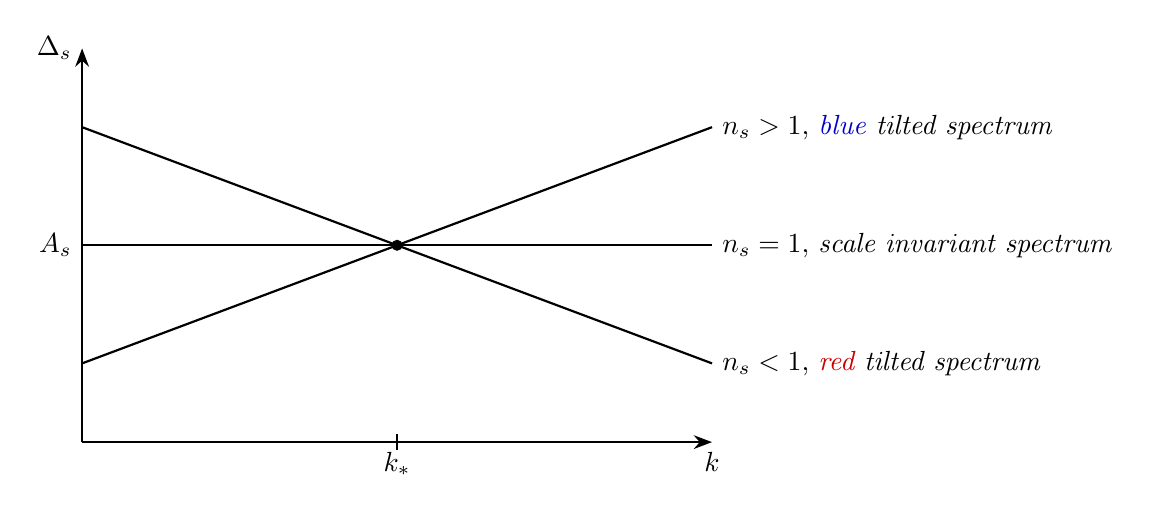
\begin{tikzpicture}[>=Stealth,thick]
    % axes
    \draw[->] (0,0) -- (8,0) node[below] {$k$};
    \draw[->] (0,0) -- (0,5) node[left] {$\Delta_s$};
  
    % central crossing point at (k*, ε_s)
    \coordinate (kp) at (4,2.5);
    \fill (kp) circle (2pt);
  
    % the three straight‐line segments
    \draw (0,4) -- (8,1);       % downward slope (n_s < 1 on right)
    \draw (0,1) -- (8,4);       % upward slope   (n_s > 1 on right)
    \draw (0,2.5) -- (8,2.5);   % horizontal      (n_s = 1)
  
    % vertical tick & label at k = k*
    \draw (4,0.1) -- (4,-0.1);
    \node[below] at (4,0) {$k_*$};
  
    % y‐axis labels
    \node[left]  at (0,2.5) {$A_s$};
  
    % labels at the right ends of each line
    \node[right] at (8,4)   {$n_s>1$, \textit{\textcolor{blue!80!black}{blue} tilted  spectrum}};
    \node[right] at (8,2.5) {$n_s=1$, \textit{scale invariant spectrum}};
    \node[right] at (8,1)   {$n_s<1$, \textit{\textcolor{red!80!black}{red} tilted  spectrum}};
  \end{tikzpicture}
\end{center}
  

\subsection{Tensor Perturbations}\label{sec:TensorPT}
They are gauge invariant as you can prove that $\tilde{h}_{ij}= h_{ij}$ (see Section~\ref{sec:cosmological_perturbation_theory}), 
\begin{equation}
    ds^2= a^2(\tau)\left[ d\tau^2  - \left(\delta_{ij} -  h_{ij}\right)  dx^i dx^j \right] = a^2(\tau)\left(\eta_{\mu\nu} + h_{\mu\nu}\right) \quad \text{with} \quad h_{\mu 0} = 0
\end{equation}
\begin{eqopt}[darkred]
    \delta G^0_0 = 0 = \delta G^0_i \qquad \delta G^i_j = \frac{1}{2a^2} \left(h^i_j{\,}'' + 2\frac{a'}{a} h^i_j{\,}' - \Delta h^i_j\right)
\end{eqopt}
In Section~\ref{sec:cosmological_perturbation_theory} we evaluated $\delta T^i_j$ of a perfect fluid/scalar field and found it was $\propto \delta^i_j$; you can check that adding $h_{ij}$ in the perturbed metric does not change this result. 
This implies $\delta G^1_1 = \delta G^2_2 = \delta G^3_3 \equiv A$, but due to the fact that $h$ is traceless (and also transverse), we have $3A = 0 \,\Rightarrow$\footnote{One can reach~\eqref{eq:EOMTP} also by expanding $S_{EH}$ action at second order in $h_{ij}$: $\frac{M_{p}^{2}}{8}\int d^{4}x\,a^{2}
\bigl[{h'_{ij}}^{2} - (\partial_{k}{h_{ij}})^{2}\bigr]$}

\begin{equation}\label{eq:EOMTP}
    h_{ij}{\,}'' + 2\frac{a'}{a} h_{ij}{\,}' - \Delta h_{ij} =0
\end{equation}
\emph{A perfect fluid does not source gravitational waves.}

$h_{ij}$ has $3(3+1)/2 -1-3 = 2$ independent components $\,\Rightarrow\, 2$ polarizations of the graviton. For propagation along $x^3$ ($h_{ij} = \epsilon_{ij}e^{ikz-i \omega\tau}$) we have
\begin{equation}
    h_{ij}= \begin{pmatrix}
        h_+ & h_x & 0\\
        h_x & -h_+ & 0 \\
        0 & 0 & 0 
        \end{pmatrix}
\end{equation}
Each polarization $h_+$, $h_x$ follows~\eqref{eq:EOMTP} and propagates at the speed of light, as there is just $c=1$ in front of $\Delta h_{ij}$.
Therefore, the action for gravitational waves can be written as:
\begin{eqopt}[darkred]
    S_{TT} = \sum_{A}\,\frac{M_{p}^{2}}{8}\int d^{4}x\,a^{2}
\bigl[(h^{(A)})'^{2} - (\partial_{k}h^{(A)})^{2}\bigr]
\end{eqopt}
Now, if we define the canonical variable
\begin{eqopt}[darkgreen]
v^{(A)} \equiv a\,h^{(A)}\frac{M_P}{2}
\end{eqopt}
we can rewrite the action as
\begin{equation}
    S_{TT} = \sum_{A}\,\frac{1}{2}\int d\tau\,d^{3}x
\bigl[(\partial_{\tau}v^{(A)})^{2}
     + \tfrac{a''}{a}\,(v^{(A)})^{2}
     - (\partial_{k}v^{(A)})^{2}\bigr]
\end{equation}
Compare it with~\eqref{eq:ScalarPTAction}, this is MS equation for tensor perturbations. The "mass" term here is $a''/a$, which is $2/\tau^2$ in dS background and $(2+3\epsilon)/\tau^2$ in slow roll background.

As in scalar case, $\int \frac{d^3k}{(2\pi)^{3/2}} v^{(A)}_{\mathbf{k}}(\tau) e^{i\mathbf{k}\cdot\mathbf{x}}$ and then solving MS equation in Fourier space leads to $v^{(A)}(\mathbf{x}, \tau) = \frac{1}{\sqrt{2}} \int \frac{d^3 k}{(2\pi)^{3/2}} \left[ a^-_k v_k^{(A)\,*}(\tau) e^{i \mathbf{k} \cdot \mathbf{x}} + a_k^+ v^{(A)}_k(\tau) e^{-i \mathbf{k} \cdot \mathbf{x}} \right]$,
we find a solution in the form of Hankel functions but with an index \textcolor{darkred}{$\nu_T = 3/2 - \epsilon$}. Imposing BD vacuum fixes constants ($C_1 = 0$, $C_2=\sqrt{\pi}/2$) and then as before we define
\begin{eqopt}[darkgreen]
\Delta_T \equiv \frac{k^3}{2\pi^2}\sum_A |h^{(A)}_k|^2 \qquad \mathcal{A}_{T} \equiv \frac{2 H^2}{\pi^2 M^2_p}\Bigg|_{k=aH}  \qquad n_T = 3-2\nu_T \textcolor{black}{\,= -2\epsilon}
\end{eqopt}
as, for slow roll ($\nu \approx 3/2$),
\begin{equation}
    \Delta_T = \frac{k^3}{2\pi^2} 2 \left(\frac{2}{a M_P}\right)^2 |v_k|^2 \approx 2 \frac{H^2}{\pi^2}\left(\frac{k}{aH}\right)^{3-2\nu}
\end{equation}
One can then define the \textit{tensor to scalar ratio} (in~\ref{sec:ScalarPT} I had $M_P = 1$)
\begin{eqopt}[darkgreen]
    r \equiv \frac{\mathcal{A}_T}{\mathcal{A}_S} \textcolor{black}{\; = 16\epsilon = -2\eta_T}
\end{eqopt}
The latter is true for all single field models and it is called \textit{consistency relation}. If observations say $r \neq -2\eta_T$ then inflation was not single field.
\subsection{Lyth Bound}\label{sec:LythBound}
Start from the fact that in flat FRW space-time $\dot{H}=-\frac{\dot{\phi}}{2M_P^2} \, \Rightarrow \, \frac{d\phi}{dN}= \sqrt{2M_P^2\epsilon}$.
\begin{equation}
    \Delta \phi = \int dN \sqrt{2M_P^2\epsilon} \approx \sqrt{2M_P^2\epsilon}\Delta N = M_P\sqrt{\frac{r}{0.01}}\sqrt{\frac{0.01}{8}}\Delta N  
\end{equation}
\begin{equation}
    \frac{\Delta \phi}{M_P} = \sqrt{\frac{r}{0.01}}\,O(1)
\end{equation}
\emph{Thus, for $r\gtrsim 10^{-2}$, $\Delta \phi > M_P \, \rightarrow$ large field inflation gives observable tensor modes,} meaning that the primordial gravitational‐wave signal it produces has an amplitude high enough 
 to be distinguished from noise in current experiments. \textcolor{blue}{$r \leq  7 \cdot 10^{-2}$}
\subsection{Observables from Inflation}\label{sec:ObsInfl}
In single‐field slow‐roll inflation the key “observables” are all evaluated at the moment each Fourier mode exits the Hubble radius during inflation. No need to know when inflation “begins” in some absolute sense. All that matters for observables is how many e-folds remain before inflation ends, because that determines when a given comoving scale $k$ crossed the Hubble radius.

In practice one picks a “pivot” wavenumber $k^* = a^* H$ (corresponding to $N^* \sim 50-60$) and defines $\mathcal{A}_s^*$, $n_s^*$, $r^*$, where $*$ means that are calculated at the pivot scale 
\begin{equation}
\log{\frac{a_{end}}{a(\phi)}}\equiv  N^* \sim \log{\frac{a_{end}H }{k^*}}
\end{equation}
Once a given mode has left the Hubble radius it “freezes in” (i.e.\ its curvature perturbation becomes conserved on superhorizon scales), so nothing in the microphysics of reheating or recombination changes the primordial values of $\mathcal{A}_s^*$, $n_s^*$, $r^*$ that were set at exit. 
\emph{What does happen between inflation and recombination is simply linear evolution through radiation and matter domination (via the transfer functions), but that evolution is completely determined by the background cosmology and does not alter the primordial spectral shape or amplitude.} Recall $\mathcal{A}_{s} \simeq 2 \cdot 10^{-9}$, $n_{s} \simeq 0.96$, $r \leq  7 \cdot 10^{-2}$.

As in Section~\ref{sec:slowRollInfl}, evaluate $\epsilon_V$, $\eta_V$ for each model. Then, get $H^* = 8 \pi^2 \epsilon A_s$ then $n_s$ and $r$.
% Large Fields Models
\begin{mycolorbox}[pink!93!black]
    \textbf{Large Fields/Monomial Models:}

    \begin{eqopt}[darkred]
       H^* \approx2.7\cdot 10^{-5} \sqrt{n}\,M_P \sim 10^5 GeV
    \end{eqopt}
    \begin{mycolorbox}[gray]
    \textbf{Duration of Inflation:}

    Approximating $H$ as constant during inflation, and using $H^* \approx2.7\cdot 10^{-5} \sqrt{n}\,M_P$
    \begin{equation}
        \Delta t = \frac{1}{H}\int_{a_{st}}^{a_{end}} \frac{d a}{a} \quad \Rightarrow \quad \Delta t \approx \frac{N}{2.7\cdot 10^{-5} \sqrt{n}M_P}\, \textcolor{darkred}{\sim 10^{-36} s}
    \end{equation}
        
    \end{mycolorbox}
\end{mycolorbox}    

% Small Fields Hill-top & Inflection Models
\begin{mycolorbox}[pink!93!black]
    \textbf{Small Fields/Hill-top \& Inflection Models:}

    Work in the regime $V_0 \gg \lambda_n \phi^n$, where you get $\eta_V \gg \epsilon_V$. Do the calculations for $n=4$.
    For slow roll models recall EOMs, in this case 
    \begin{equation}
        H^2 = \frac{1}{3M^2_P} \left(\frac{\dot{\phi}^2}{2} + V\right)  \sim \frac{V_0}{3}
    \end{equation}
    With this you can evaluate $A_s$ and the fix $\lambda$, you have only $V_0$ as free parameter.

\end{mycolorbox}

% Plateau Models
\begin{mycolorbox}[pink!93!black]
    \textbf{Plateau Models:}

   For $n_s$ discard $1/N^2$ term. For Starobinsky model ($\alpha=1, k=\sqrt{2/3}$) we have excellent agreement ($r \approx 0.004$).
\end{mycolorbox}

\section{The last scattering surface}\label{sec:LST}
\emph{When inflation ends the inflaton dumps its energy into standard model particles:} this is the process called \textit{reheating}. 
After reheating the Universe is still radiation dominated until recombination at $t_{eq}$. The latter time can be estimated, in terms of redshift $z_{eq}$, by $\rho_m^{eq} = \rho_\gamma^{eq}$ and then employing $\Omega_{\rho_i}^{\text{now}}$.

After radiation-matter equivalence the Universe remains a coupled baryon-photon plasma until recombination, when the already existing free photons can propagate freely; resulting in Plankian spectrum we observe: the CMB.

To estimate $z_{rec}$ start from the number density of a certain species
\begin{eqopt}[darkred] \label{eq:NumberDensityExact}
    n=\frac{g}{(2\pi)^3}\int f(\mathbf{p}) d^3p \; \textcolor{black}{=\, \frac{g}{2\pi^2}\int_m^\infty f(\mathbf{E}) E \sqrt{E^2-m^2} dE} \qquad f(\mathbf{p})= \frac{1}{e^{\frac{E-\mu}{T}}\pm 1}
\end{eqopt}
Approx $e^{\frac{E-\mu}{T}}\pm 1 \approx e^{\frac{E-\mu}{T}}$ and consider non-relativistic particles, for which $T\ll m$:
\begin{eqopt}[darkred]\label{eq:NumberDensityApprox}
    n=g\left(\frac{mT}{2\pi}\right)^{3/2}\,e^{\frac{\mu - m}{T}}
\end{eqopt}
$g = 2 S +1$-factors are the usual internal degeneracy (spin, etc.) of each species.
The \textit{proton-electron capture} to form neutral hydrogen is the process happening at recombination. In the early Universe before recombination we have equilibrium: $p + e \leftrightarrow  H + \gamma$.
\underline{Assume $n_B = n_p + n_H$}, i.e.\ all baryons are in the form of protons and hydrogen atoms. \underline{Assume thermal and chemical ($\mu_H = \mu_p + \mu_e$) equilibrium}. Furthermore, $n_p = n_e$ due to charge neutrality.
We are interested in the ratio $n_H / (n_p n_e) $ as it tells us how neutral (and thus transparent for photons) is the Universe at temperature $T$. Define \textit{hydrogen biding energy} \textcolor{darkgreen}{$B\equiv m_p+m_e -m_H$}. Employing~\eqref{eq:NumberDensityApprox}
\begin{equation}\label{eq:SahaInitial}
    \frac{n_H}{n_pn_e}\, \overset{m_H \simeq m_p}{\approx}\, \underbrace{\frac{g_H}{g_p g_e}}_{=1} \left(\frac{2\pi}{m_e T}\right)^{3/2} e^{B/T} \overset{!}{=} \frac{n_p /n_B^2}{n_e^2/n_B^2} = \frac{1}{n_B} \frac{1-n_e/n_B}{n_e^2/n_B^2}
\end{equation}
Define the \textit{fractional ionization} \textcolor{darkgreen}{$ \chi_e \equiv n_e / n_B$} and the \textit{baryon to photon ratio} \textcolor{darkgreen}{$ \eta \equiv n_B / n_\gamma$}\textcolor{blue}{$\,\simeq 6\cdot 10^{-10}$}. Where \textcolor{darkred}{$n_\gamma = \frac{2}{\pi^2} \zeta(3)T^3$} comes from direct integration of~\eqref{eq:NumberDensityExact}.
We can now rewrite~\eqref{eq:SahaInitial} in the form called \textit{Saha equation}
\begin{eqopt}\label{eq:Saha}
    \frac{1-\chi_e}{\chi_e^2}\Bigg|_{eq} = \frac{4\sqrt{2}}{\sqrt{\pi}}\zeta(3) \eta \left(\frac{T}{m_e}\right)^{3/2} e^{B/T}
\end{eqopt}
Universe becomes transparent for $\chi_e \rightarrow 0$, as free protons and electrons diminish and the former start having a  high mean free path.
\textcolor{darkred}{For $\chi_e = 0.01$ we have from~\eqref{eq:Saha} $T \approx 3500K$} $\; \Rightarrow z_{rec}=\frac{T_{rec}}{T_{now}}-1 \simeq 1200$.

Thermal equilibrium is no longer a good approximation during inflation, indeed a more accurate result can be found using kinetic theory: \textcolor{darkred}{$z_{rec}\simeq1100$}.
\subsection{Introducing CMB temperature anisotropies}\label{sec:CMBAnisotropies}
To study how photons propagate between last scattering surface (LSS) and today consider a flat Universe subject to scalar perturbations (here $\Psi \neq -\Phi$ as we are not working in single perfect fluid approximation), change sign of $\Psi$ for convenience:
\begin{equation}
    ds^2 = a^2(\tau)\left[\left(1+2\Phi\right)d\tau^2 - \left(1+2\Psi\right) \delta_{ij} dx^idx^j\right]
\end{equation}
Write down geodesic equation for photons, first with affine parameter $\lambda$, then in conformal time.
\begin{equation}
    \dot{P}^\beta + \Gamma^\beta_{\mu\nu}P^\mu P^\nu = 0 \qquad P^\mu= \frac{dx^\mu}{d \lambda} \qquad \dot{P}^\mu= \frac{dP^\mu}{d \lambda} = \frac{dP^\mu}{d \tau} P^0
\end{equation} 
Look at $0$ component and then compute full perturbed connections at first order, in doing so expand $(1+2\Phi)^{-1}$:
\begin{equation}
   \frac{dP^0}{d \tau} + \Gamma^0_{\mu\nu}\frac{P^\mu P^\nu}{P^0} = 0 
\end{equation}
Plug the expressions in and use the null condition $P^{\mu}P_{\nu}=0$ to get $P^i = P^0 \left(1+\Phi -\Psi \right) n^i$ 
Where $n^i$ is any unit vector on the sphere (pointing along photon's direction in the comoving spatial frame).
\begin{figure}[h] 
      \centering  
        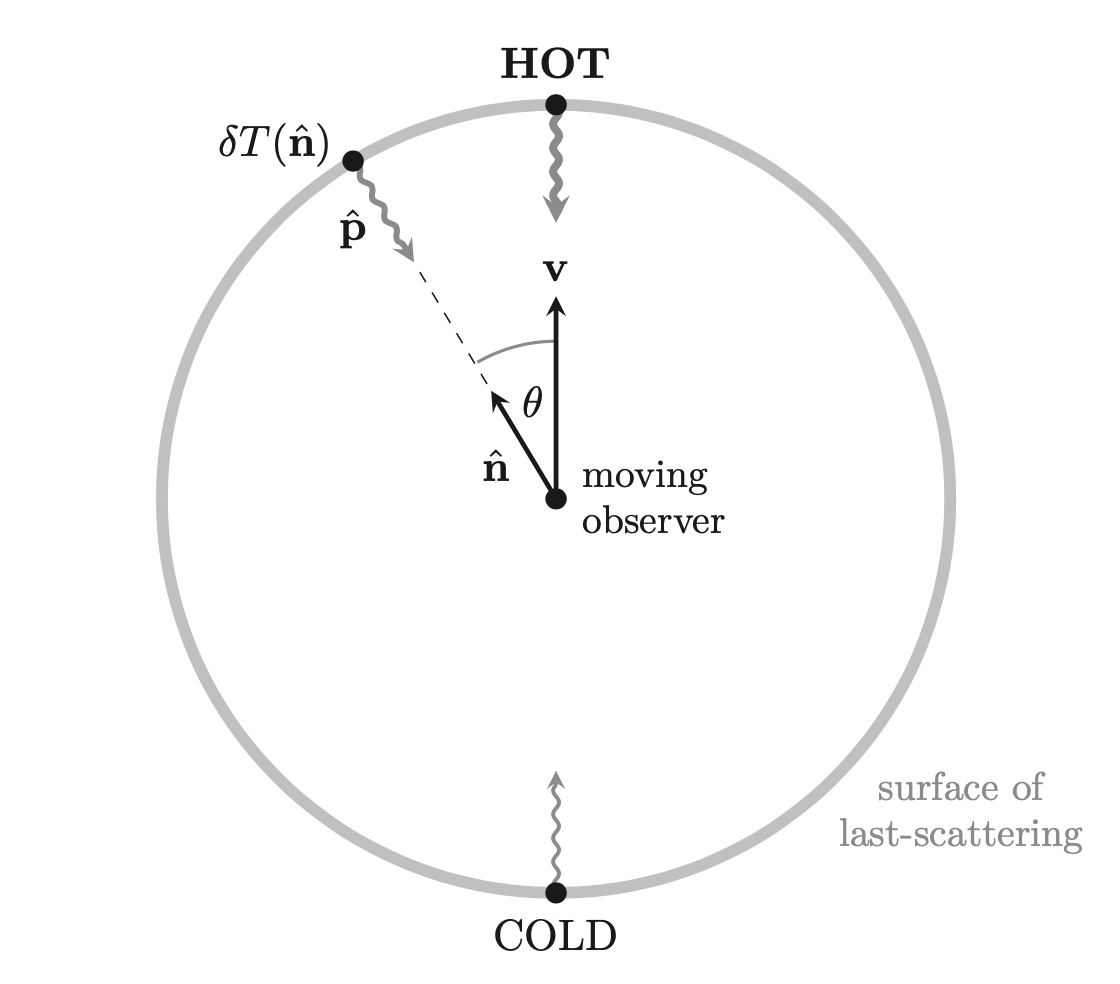
\includegraphics[width=0.8\textwidth]{Graphics/CMB-doppler.png}
        \caption{Motion of the Solar System relative to CMB rest frame~\cite{CosmologyBau}.}
  \end{figure}
This leads to\footnote{Recall $'$ are \emph{partial} derivatives with respect to $\tau$.}
\begin{equation}\label{eq:0thcomponentGeo}
    \frac{dP^0}{d \tau} + 2\frac{a'}{a}P = -P^0 \left(\Psi'+\Phi'\right) -2\Phi_{,i}n^i P^0 
\end{equation}
Define the \textit{conformal momenta} \textcolor{darkgreen}{$\varTheta^\mu \equiv  a^2 P^\mu $} to notice that $\varTheta^0$ is conserved at zeroth order! This means that 
\emph{different photons of different frequency get red-shifted in the same way} $\,\Rightarrow\,$ the spectrum keeps its shape (at zeroth order).

Notice that the \emph{total} derivative of $\tau$ on $\Phi(\tau,x^i) = \Phi'+ \Phi_{,i} \tfrac{P^i}{P^0}$, so you can rewrite~\eqref{eq:0thcomponentGeo} as
\begin{equation}
    \frac{d\varTheta^0}{d \tau} = \varTheta^0 \left[\left(\Phi' - \Psi' \right) - 2  \frac{d\Phi}{d\tau}\right]
\end{equation}
This can be integrated and then expanded around $\varTheta^0(\tau'') \sim  \varTheta^0(\tau')$ (motivated by the consideration above).
\begin{equation}\label{eq:momentaShifts}
    \frac{\Theta^{0}(\tau'')-\Theta^{0}(\tau')}{\Theta^{0}(\tau')} = - 2\left[\Phi(\tau'')-\Phi(\tau')\right] + \int_{\tau'}^{\tau''} \left(\Phi'-\Psi'\right)d\tau 
\end{equation}

The four momentum components $P^\mu=(P^0,P^i)$ are defined in the
coordinate frame, while what an observer actually measures as the photon energy
and momentum are the components $P^{\hat{\mu}}=(E,P^{\hat{i}})$ in their local inertial frame. \underline{Assume that the observer is comoving} \underline{with the cosmic fluid.}
To get the relative frequency shift from~\eqref{eq:momentaShifts}, consider $E=U_\mu P^\mu$ and get $U_\mu$ from $U^\mu U_\mu = 1$.
\begin{equation}
    E = aP^{0}\left(1+\Phi-\mathbf{n}\cdot\mathbf{\delta v}\right)
\end{equation}
So that, if we multiply both sides by $a(\tau)$ we construct $\varTheta$:
\begin{equation}
    \frac{\Theta^{0}(\tau'')-\Theta^{0}(\tau')}{\Theta^{0}(\tau')} = \frac{E a(\tau'')}{E a(\tau')}\Bigl[1-\Phi(\tau'')+\mathbf{n}\cdot \delta\mathbf{v}(\tau'')+\Phi(\tau')-\mathbf{n} \cdot \delta\mathbf{v}(\tau')\Bigr] - 1
\end{equation}
Now we wish to expand $E(\tau'')$, to do so first notice that $E(\tau'')a(\tau'')=E(\tau')a(\tau')$ at zeroth order. Hence $E(\tau'')a(\tau'') \sim \left[E(\tau')+ \Delta E(\tau'',\tau')\right]a(\tau')\,$. The relative frequency shift for a photon emitted at $\tau'$ and detected at $\tau''$ is thus
\begin{equation}\label{eq:photonEnergyShift}
    \frac{\Delta E(\mathbf{n},\tau'',\tau')}{E(\tau')} = \Phi(\tau')- \Phi(\tau'') +  \mathbf{n} \cdot \delta\mathbf{v}(\tau') -\mathbf{n}\cdot \delta\mathbf{v}(\tau'') + \int_{\tau'}^{\tau''} \left(\Phi'-\Psi'\right)d\tau 
\end{equation}
Notice that \emph{so far we only computed $\Delta E$, which is the change in the energy of a single photon along its geodesic, we are now interested in $\delta T$: the change in the local blackbody temperature of a whole ensemble of photons at last scattering.} 

Consider an ensemble of photons with temperature $T$ and set $\tau''=\tau_{now}$, $\tau'=\tau_{rec}$. Temperature and energy redshift the same way, therefore a fractional change in photon energy is exactly the same as a fractional change in the blackbody temperature you would assign to the beam. Now we have also to add an “intrinsic” piece due to local density perturbations in the ensemble (recalling $\rho_\gamma \propto T^4$).
You can absorb the \textit{monopole term} $\Phi(\tau_{now})$ into the average temperature\footnote{CMB experiments only measure differences in temperature: $\Delta T(\mathbf{n})= T(\mathbf{n}) - T_{avg}$, thus, adding a constant to every photon’s energy (or to the mean temperature) simply shifts the zero-point of $T$.}
and neglect the \textit{dipole term} $\mathbf{n} \cdot \delta\mathbf{v}(\tau_{now})$ as it accounts for the Doppler effect due to the relative motion of the observer with respect to the CMB rest frame\footnote{It comes from our local motion, not from fluctuations at recombination or along the line of sight; we subtract it in data processing: experiments fit and remove the dipole to isolate the cosmological signal.}.
\begin{eqopt}\label{eq:SachsWolfe}
    \frac{\delta T}{T}\left(\mathbf{n},\tau_{now}\right)
= \frac{\delta \rho_\gamma}{4\rho_\gamma}(\tau_{rec})
   + \Phi(\tau_{\rm rec})+ n^{i}v_{i}(\tau_{\rm rec})
  + \int^{\tau_{now}}_{\tau_{\rm rec}}\!(\Phi'-\Psi')\,d\tau
\end{eqopt}
This is the \textit{Sachs-Wolfe equation}, which states that the observed temperature anisotropies originate from 
\begin{itemize}
\item Intrinsic density fluctuations at LSS 
\item Fluctuations of gravitational potential (gravitational red/blue shift) at LSS 
\item Doppler effects at LSS 
\item Contributions from time varying gravitational potential between LSS and detection
\end{itemize}
\emph{CMB pattern is generated by sending photons from the last‐scattering surface (at recombination) to us, through an inhomogeneous universe. 
The shift in energy of~\eqref{eq:photonEnergyShift} is direction dependent (due to $\Phi$, $\Psi$ and $\mathbf{n}\cdot \delta\mathbf{v}$), so it imprints a spatial anisotropy in the observed photon energies.}
\begin{eqopt}[blue]
    \frac{T(\mathbf{n})-T^{avg}_{now}}{T^{avg}_{now}} \sim 10^{-4}- 10^{-5}
\end{eqopt}
\subsection{CMB temperature anisotropies: multipoles}\label{sec:CMBMultipoles}
The temperature anisotropy in the $\mathbf{n}$ direction in the sky is a square-integrable function on the sphere and thus can be expanded in terms of spherical harmonics
\begin{eqopt}[darkred]\label{eq:harmonicExpansion}
    \frac{\delta T_{now}}{T_{now}}(\mathbf{n}) = \sum_{l=1}^\infty\sum_{m=-l}^{l} a_{lm}Y_{lm}(\mathbf{n})
\end{eqopt}
Using common conventions, we introduce spherical harmonics and (associated) Legendre polinomials as follows:
\begin{eqopt}[darkgreen]
    Y_{l}^m(\theta ,\varphi)=(-1)^m \sqrt{\frac{2l+1}{4\pi} \frac{(l-m)!}{(l+m)!}}\,e^{im\phi}\,P_{l}^m(\cos{\theta}) \qquad P_{l}^{-m} = (-1)^m\frac{(l-m)!}{(l+m)!} P_{l}^{m}
\end{eqopt}
It follows that $ {Y_{l}^m}^* = (-1)^m Y_{l}^{-m}$ and, from~\eqref{eq:harmonicExpansion}, $a^*_{lm}=(-1)^m a_{l-m}$. It also follows that
\begin{eqopt}[darkred]
    \int_0^{\pi} d\theta \int_{0}^{2\pi}  Y_{l}^m Y_{l'}^{-m'} sin(\theta) d\theta d\phi = \delta_{ll'} \delta_{mm'}
\end{eqopt}
We can use this orthonormality to determine the \textit{multipole moments} $a_{lm}$:
\begin{equation}
    a_{lm}=\int d\mathbf{n} \frac{\delta T_{now}}{T_{now}}(\mathbf{n}) Y^*_{lm}(\mathbf{n})
\end{equation}

The CMB \textit{angular power spectrum} $C_l$ we obtain experimentally is the ensemble two-point function of the $a_{lm}$.  One then considers an average over all possible realizations of the Universe (a hypothetical average over infinitely many CMB skies)\footnote{Not to be confused with the inner product on the 2-sphere, which decomposes \emph{one} sky map into modes.}
\begin{equation}\label{eq:ensembleAverage}
    \bigl<a_{lm}a^*_{l'm'} \bigr>=C_l \,\delta_{ll'}\,\delta_{mm'} \qquad \hat{C}_l = \frac{1}{2l+1} \sum_{m=-l}^l \abs{a_{lm}}^2 \approx C_l
\end{equation}
The introduction of an \textit{estimator} $\hat{C}_l$ for $C_l$ is motivated due to the fact that, for fixed $l$, we have $2l+1$ different $a_{lm}$, allowing for $2l+1$ independent estimated of $C_l$.
Because the process is assumed statistically isotropic, all the $2l+1$ different $m$-modes at fixed $l$ are statistically equivalent, hence averaging over them in our one sky gives an unbiased estimator of the ensemble-average power~\cite{CosmologyBau}.
$\hat{C}_l = C_l$ in the infinite ensemble limit, i.e.\ $\bigl<\hat{C}_l \bigr>=C_l$. However, we have a nonzero \textit{cosmic variance}
\begin{eqopt}[darkred]
    \frac{\Delta C_l}{C_l}= \sqrt{\frac{2}{2l+1}}
\end{eqopt}
which can be proved using Wick's theorem in quite a long calculation starting from $\Delta C_l \equiv \sqrt{\bigl<(C_l-\hat{C}_l)^2 \bigr>}$ . We thus have large errors for small $l$ values.
\begin{comment}
If you look at a single $l$ pattern on the sky, you'll see alternating rings (for $m =0$) or lobes (for $m \neq0$).
The Legendre polinomials $P_l^0 (\cos{\theta})$ have exactly $l$ zeros in the interval $0,\pi$, the first one is $\theta \sim \pi /2l$, a full oscillation of the pattern (hot $\rightarrow$ cold $\rightarrow$ hot) on the sphere takes two of those zero-crossings, i.e.\ an angular period $\Delta \theta \sim \pi/l$.
Therefore, for large $l$, a multipole $l$ corresponds to a small angular scale and statistics gets better (as sample scales as $2l+1$).
\end{comment}
 
The CMB temperature fluctuations are analyzed statistically by measuring the correlations
between hot and cold spots as a function of their angular separation.
\begin{figure}[h]
      \centering
        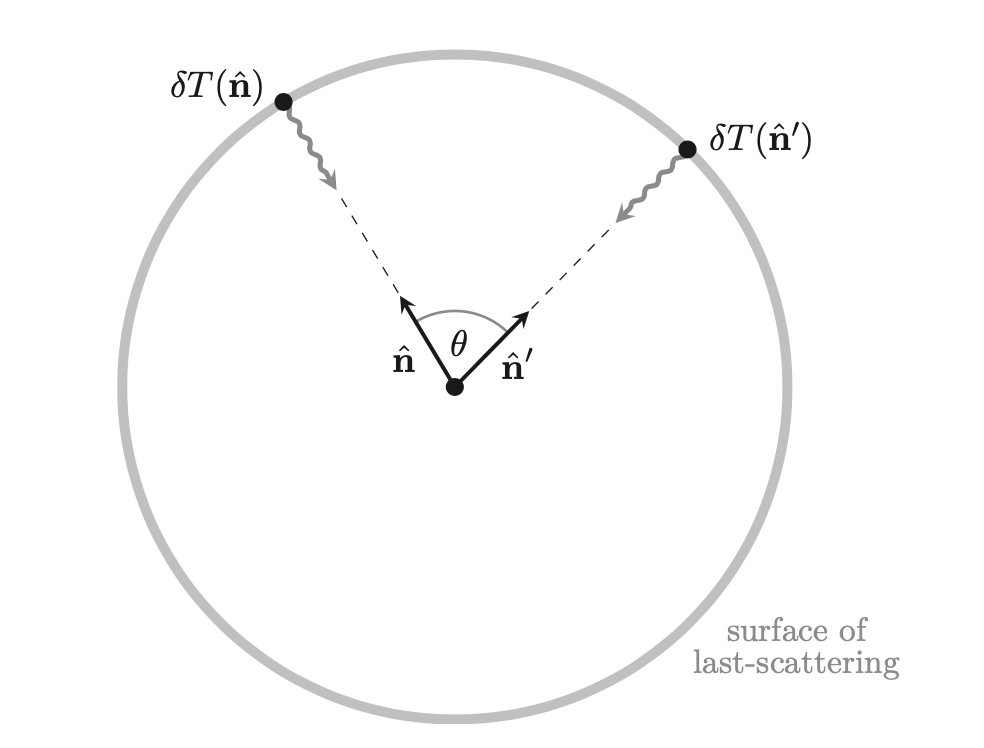
\includegraphics[width=0.8\textwidth]{Graphics/CMB-2point.png}
        \caption{2-point correlations $\bigl<\frac{\delta T}{T} (\mathbf{n})\frac{\delta T}{T} (\mathbf{n}')\bigr>$ between temperature fluctuations on LSS~\cite{CosmologyBau}.}
  \end{figure}
  Employing the \textit{addition theorem},
  \begin{eqopt}[darkred]\label{eq:additionTh}
     \sum_{m=-l}^l Y^m_l(\mathbf{n}){Y^m_l}^*(\mathbf{n}') = \frac{2l+1}{4\pi} P_l Y^m_l(\mathbf{n}\cdot\mathbf{n}')
  \end{eqopt}  
  It is easy to show that 
  \begin{equation}
    \bigl<\frac{\delta T}{T} (\mathbf{n})\frac{\delta T}{T} (\mathbf{n}')\bigr> = \sum_{ll'}\sum_{mm'}\bigl<a_{lm}a_{l'm'}^* \bigr>Y^m_l(\mathbf{n}) Y^{m'}_{l'}(\mathbf{n}') =\sum_l C_l \frac{2l+1}{4\pi} P_l(\mathbf{n}\cdot\mathbf{n}')
  \end{equation}
  For large $l$, setting $\mathbf{n} = \mathbf{n}'$ $(P_l(1)=1 \quad \forall\, l)$,
  \begin{equation}
  \bigl<\frac{\delta T}{T} (\mathbf{n})\frac{\delta T}{T} (\mathbf{n}')\bigr> \approx \int d\log{l} \frac{l^2+1}{2\pi}C_l
  \end{equation}
  One usually plots the CMB power spectrum as
  \begin{eqopt}[darkgreen]
    \mathcal{D}_l \equiv T_0^2 \frac{l(l+1)}{2\pi}C_l
  \end{eqopt}
  \vspace{-0.6cm}
  
  We now want to express the angular power spectrum in terms of perturbations during inflation.
  Using~\eqref{eq:ensembleAverage}~\eqref{eq:harmonicExpansion}~\eqref{eq:additionTh} we get 
  \begin{equation}
    C_l =\frac{1}{4\pi} \int d\mathbf{n} d\mathbf{n}' \bigl<\frac{\delta T}{T} (\mathbf{n})\frac{\delta T}{T}^* (\mathbf{n}')\bigr> P_l(\mathbf{n}\cdot\mathbf{n}')
  \end{equation}
  Then \underline{assume instantaneous recombination}, i.e.\ infinitely small LSS, and expand $\frac{\delta T}{T}$ in Fourier space with a further expansion of a plane wave in terms of Legendre polinomials. A rather technical derivation brings to
\begin{eqopt}
    C_l = \frac{2}{\pi}\int dk k^2 P_{\Phi}(k) \underbracket{\tilde{\frac{\delta T}{T}}(k) \tilde{\frac{\delta T}{T}}^*(k) \left[j_l(k r_*)\right]^2}_{\text{transfer function}}
\end{eqopt}
where $ P_{\Phi}(k) \delta^{(3)}(\mathbf{k}+\mathbf{k}')\equiv \bigl<\Phi(\mathbf{k}) \Phi^*(\mathbf{k}') \bigr> $ is a primordial spectrum contribution coming from the power spectrum of scalar perturbations at recombination, while $\tilde{\frac{\delta T}{T}}(k)$ is defined to be independent of the gravitational field: $\frac{\delta T}{T} = \tilde{\frac{\delta T}{T}} \Phi$; $j_l$ is a spherical Bessel function ($r_*$ is the comoving radial distance from us to LSS).
The transfer function is determined by~\eqref{eq:SachsWolfe}.
\subsection{CMB temperature anisotropies: Sachs-Wolfe plateau}\label{sec:CMBSWPlateau}
Consider perturbations that are superhorizon at recombination, $k\tau_{rec}<1$. Recall that in Section\ref{sec:SingCompFluid} we showed that $\delta \rho_m /\bar{\rho}_m = -2\Phi$ on superhorizon scales in a matter dominated Universe.
On scales much larger than the horizon, causally disconnected regions can’t “talk” to one another. Each patch evolves as if it were its own exact FRW cosmos, with its own scale factor, densities, pressures etc.
Instead of every patch having precisely the same cosmic time $t$ you say patch $\mathbf{x}$ has time $t+\delta t(\mathbf{x})$. \emph{The perturbation doesn’t come from heat flow or exchange with the outside, but from the fact that inflation left some regions a little “ahead” or “behind” in their evolution.}
\underline{Assume that the perturbation is adiabatic} $\,\Rightarrow\,$ all species share the same clock shift, therefore
\begin{equation}
    \frac{\delta \rho^i}{(\rho^i+p^i) } = -3H \delta t \quad \text{same }\forall i \quad \Rightarrow \quad \frac{\delta \rho_m}{(\rho_m+p_m) } =\frac{\delta \rho_\gamma}{(\rho_\gamma+p_\gamma) } =\frac{3}{4}\frac{\delta \rho_\gamma}{\rho_\gamma} 
\end{equation}
and thus, at recombination (when Universe is matter dominated), $\frac{\delta \rho_\gamma}{\rho_\gamma} = -\frac{8}{3}\Phi$.

For these modes, Sachs-Wolfe equation can be approximated by ignoring Doppler and time varying potential contribution:
\begin{equation}
    \frac{\Delta T_{now}}{T_{now}} (\mathbf{n}) \approx \frac{\delta \rho_\gamma}{4} (\tau_{rec}) + \Phi (\tau_{rec})= \frac{1}{3}\Phi
\end{equation}

Again from Section~\ref{sec:SingCompFluid}, recall that $\Phi_{\mathrm{matter}} = (9/10) \Phi_{\mathrm{rad}} \, \Rightarrow \, \Phi(\tau_{rec})=(9/10)\Phi(\tau_{infl})$, as $\Phi(\tau_{infl}) \equiv \Phi(\tau_{i})$ is constant on superhorizon scales.
\begin{center}
    \begin{tikzpicture}
  \begin{axis}[
    width=10cm, height=5cm,
    xlabel={$\tau$},
    ylabel={$\Phi(\tau)$},
    ymin=0, ymax=1.2,
    xmin=0, xmax=4, 
    xtick={1.5,3},
    xticklabels={$\tau_{\rm eq}$,$\tau_{\rm rec}$},
    ytick={0.7,1},
    yticklabels={$\tfrac{9}{10}\,\Phi(\tau_i)$,$\Phi(\tau_i)$},
    domain=0:4,
    axis lines=middle, 
    clip=false,
  ]
    % initial plateau at unity
    \addplot[black, thick] coordinates {(0,1) (1.5,1)};
    % step down
    \addplot[black, thick] coordinates {(1.5,1) (1.5,0.7)};
    % second plateau
    \addplot[black, thick] coordinates {(1.5,0.7) (4,0.7)};
  \end{axis}
\end{tikzpicture}
\end{center}
Therefore, 
\begin{equation}
     \frac{\Delta T_{now}}{T_{now}} (\mathbf{n}) \approx \frac{3}{10}\Phi(\tau_i) = \frac{3}{10} \int \frac{d^3k}{(2\pi)^{3/2}}\Phi(\mathbf{k},\tau_i) e^{i \mathbf{k}\mathbf{n}r_*}
\end{equation}
As before expand the plane wave in Legendre polinomials to reach
\begin{eqopt}[darkred]\label{eq:ClApprox}
    C_l = \frac{36 \pi}{100} \int \frac{dk}{k} \Delta_{\Phi}(k) j^2_l (k r_*)
\end{eqopt}
with \textcolor{darkgreen}{$\Delta_{\Phi}(k) \equiv \frac{k^3}{2 \pi^2} P_{\Phi}(k)$}. Then define \textcolor{darkgreen}{$\Delta_{\Phi}(k) \equiv \left(\frac{k}{k_*}\right)^{n_s-1} \mathcal{A}_{\Phi}$}. With \textcolor{darkred}{$n_s \approx 1$}~\eqref{eq:ClApprox} can be integrated to get 
\begin{eqopt}[darkred]
    C_l=\frac{18 \pi}{100} \frac{\mathcal{A}_\Phi}{l(l+1)}
\end{eqopt}
CMB data yelds
\begin{eqopt}[blue]
    \frac{l(l+1)C_l}{2\pi} \sim 10^{-10} \quad\textcolor{black}{\Rightarrow \quad \mathcal{A}_\Phi \approx 10^{-9}}
\end{eqopt}

We can use this bound to constrain the scale of inflation. Define the \textit{uniform density curvature perturbation} $\mathcal{\xi}$ as the curvature perturbation measured on hypersurfaces where the total energy density is unperturbed:
\begin{eqopt}[darkgreen]
   \mathcal{R} \equiv -\Phi - \frac{H}{\dot{\phi}}\delta \phi \qquad \mathcal{\xi} \equiv -\Phi + \frac{3(\delta \rho)}{\rho+p} 
\end{eqopt}
Notice that, on superhorizon scales, the comoving curvature perturbation $\mathcal{R}=u/z$ is $\approx\mathcal{\xi}= -\frac{3}{2}\Phi$ (in radiation dominated Universe as it is during inflation).  
We can also define the dimensionless power spectrum of $\mathcal{R}$ in the usual way: $\Delta_{\mathcal{R}} \equiv \frac{k^3}{2\pi^2} P_{\mathcal{R}_k} =\left(\frac{k}{k_*}\right)^{n_s-1} \mathcal{A}_{\mathcal{R}}$.
\begin{equation}
    \mathcal{R} \approx \mathcal{\xi}= -\frac{3}{2}\Phi \quad \Rightarrow \quad \Delta_{\mathcal{R}} = \frac{9}{4} \Delta_{\Phi} \quad \Rightarrow \quad \mathcal{A}_{\mathcal{R}} = \frac{9}{4}  \mathcal{A}_\Phi \approx 2\cdot 10^{-9}
\end{equation}
This implies $H\simeq 10^{-4} \sqrt{\epsilon} \,M_P$

% ********************************** Bibliography ******************************
\begin{spacing}{0.9}

\cleardoublepage 
\nocite{*} 
\printbibliography[heading=bibintoc, title={References}]
\thispagestyle{empty}
\end{spacing}
\end{document}
